% *************************************************************************************************************************
% *************************************         SOLUCION                      *********************************************
% *************************************************************************************************************************


% =======================================================
% =======         HEADER FOR DOCUMENT        ============
% =======================================================
    
    % *********   DOCUMENT ITSELF   **************
    \documentclass[12pt, fleqn]{report}                             %Type of doc and size of font and left equations
    \usepackage[margin=1.2in]{geometry}                             %Margins and Geometry pacakge
    \usepackage{ifthen}                                             %Allow simple programming using if - then
    \usepackage[hidelinks]{hyperref}                                %Allow to create hiperlinks and Fuck Firefox
    \usepackage{pdfpages}                                           %Allow us 'import' PDF's
    \hypersetup{pageanchor=false}                                   %Solve 'double page 1' warnings in build :v
    \setlength{\parindent}{0pt}                                     %Eliminate ugly indentation
    \author{Jose Luis Onofre Franco y Oscar Andres Rosas Hernandez} %Who I am

    % *********   LANGUAJE    *****************
    \usepackage[spanish]{babel}                                     %Please allow me to type in spanish
    \usepackage[utf8]{inputenc}                                     %Lets use UFT-8
    \usepackage[T1]{fontenc}                                        %Allow for better font support
    \usepackage{textcmds}                                           %Allow us to use quoutes
    \usepackage{changepage}                                         %Allow us to use identate paragraphs
    \usepackage{anyfontsize}                                        %All the sizes for fonts wiiiii!

    % *********   MATH AND HIS STYLE  *********
    \usepackage{ntheorem, amsmath, amssymb, amsfonts}               %All fucking math, I want all!
    \usepackage{mathrsfs, mathtools, empheq}                        %All fucking math, I want all!
    \usepackage{cancel}                                             %Negate symbol
    \usepackage{centernot}                                          %Allow me to negate a symbol
    \decimalpoint                                                   %Use decimal point

    % *********   GRAPHICS AND IMAGES *********
    \usepackage{graphicx}                                           %Allow to create graphics
    \usepackage{float}                                              %For images
    \usepackage{wrapfig}                                            %Allow to create images
    \graphicspath{ {Graphics/} }                                    %Where are the images :D

    % *********   LISTS AND TABLES ***********
    \usepackage{listings, listingsutf8}                             %We will be using code here
    \usepackage[inline]{enumitem}                                   %We will need to enumarate
    \usepackage{tasks}                                              %Horizontal lists
    \usepackage{longtable}                                          %Lets make tables awesome
    \usepackage{booktabs}                                           %Lets make tables awesome
    \usepackage{tabularx}                                           %Lets make tables awesome
    \usepackage{multirow}                                           %Lets make tables awesome
    \usepackage{multicol}                                           %Create multicolumns

    % *********   REMOVE SOME ERRORS **********
    \hbadness=10000                                                 %Ignore \vbox and \hbox warings
    \hfuzz=\maxdimen\newdimen\hfuzz                                 %Ignore \vbox and \hbox warings

    % *********   HEADERS AND FOOTERS ********
    \usepackage{fancyhdr}                                           %Lets make awesome headers/footers
    \pagestyle{fancy}                                               %Lets make awesome headers/footers
    \setlength{\headheight}{16pt}                                   %Top line
    \setlength{\parskip}{0.5em}                                     %Top line
    \renewcommand{\footrulewidth}{0.5pt}                            %Bottom line

    \lhead {                                                        %Left Header
        \hyperlink{chapter.\arabic{chapter}}                        %Make a link to the current chapter
        {\scriptsize{\textsc{\nouppercase{\leftmark}}}}             %And fot it put the name
    }

    \rhead {                                                        %Right Header
        \hyperlink{section.\arabic{chapter}.\arabic{section}}       %Make a link to the current chapter
            {\scriptsize{\textsc{\nouppercase{\rightmark}}}}        %And fot it put the name
    }

    \rfoot{\textsc{\scriptsize{\hyperref[sec:Index]{Ve al Índice}}}}%This will always be a footer  

    \fancyfoot[L]{                                                  %Algoritm for a changing footer
        \ifthenelse{\isodd{\value{page}}}                           %IF ODD PAGE:
            {\scriptsize{\textsc{Oscar Andres Rosas Hernandez}}}    %Send the page
            {\scriptsize{\textsc{Jose Luis Onofre Franco}}}         %Send the author
    }
    
    
% =======================================================
% ===================   COMMANDS    =====================
% =======================================================

    % =========================================
    % =======   NEW ENVIRONMENTS   ============
    % =========================================
    \newenvironment{Indentation}[1][0.75em]                         %Use: \begin{Inde...}[Num]...\end{Inde...}
        {\begin{adjustwidth}{#1}{}}                                 %If you dont put nothing i will use 0.75 em
        {\end{adjustwidth}}                                         %This indentate a paragraph
    
    \newenvironment{SmallIndentation}[1][0.75em]                    %Use: The same that we upper one, just 
        {\begin{adjustwidth}{#1}{}\begin{footnotesize}}             %footnotesize size of letter by default
        {\end{footnotesize}\end{adjustwidth}}                       %that's it
    
    \def \Eq {equation}                                             %Stupid Visual studio error
    \newenvironment{MultiLineEquation}[1]                           %Use: To create MultiLine equations
        {\begin{\Eq}\begin{alignedat}{#1}}                          %Use: \begin{Multi..}{Num. de Columnas}
        {\end{alignedat}\end{\Eq}}                                  %And.. that's it!
    
    \newenvironment{MultiLineEquation*}[1]                          %Use: To create MultiLine equations
        {\begin{\Eq*}\begin{alignedat}{#1}}                         %Use: \begin{Multi..}{Num. de Columnas}
        {\end{alignedat}\end{\Eq*}}                                 %And.. that's it!
    

    % =========================================
    % == GENERAL TEXT & SYMBOLS ENVIRONMENTS ==
    % =========================================
    
    % =====  TEXT  ======================
    \newcommand \Quote              {\qq}                           %Use: \Quote to use quotes
    \newcommand \Over               {\overline}                     %Use: \Bar to use just for short
    \newcommand \ForceNewLine       {$\Space$\\}                    %Use it in theorems for example
    \newcommand \ForceColumnBreak   {\vfill\null\columnbreak}       %Use only in multicols

    % =====  SPACES  ====================
    \DeclareMathOperator \Space     {\quad}                         %Use: \Space for a cool mega space
    \DeclareMathOperator \MegaSpace {\quad \quad}                   %Use: \MegaSpace for a cool mega mega space
    \DeclareMathOperator \MiniSpace {\;}                            %Use: \Space for a cool mini space
    
    % =====  MATH TEXT  =================
    \newcommand \Such           {\MiniSpace | \MiniSpace}           %Use: \Such like in sets
    \newcommand \Also           {\MiniSpace \text{y} \MiniSpace}    %Use: \Also so it's look cool
    \newcommand \Remember[1]    {\Space\text{\scriptsize{#1}}}      %Use: \Remember so it's look cool
    
    % =====  THEOREMS: IN SPANISH :0  ===
    \newtheorem{Theorem}        {Teorema}[section]                  %Use: \begin{Theorem}[Name]\label{Nombre}...
    \newtheorem{Corollary}      {Colorario}[Theorem]                %Use: \begin{Corollary}[Name]\label{Nombre}...
    \newtheorem{Lemma}[Theorem] {Lemma}                             %Use: \begin{Lemma}[Name]\label{Nombre}...
    \newtheorem{Definition}     {Definición}[section]               %Use: \begin{Definition}[Name]\label{Nombre}...
    \theoremstyle{break}                                            %THEOREMS START 1 SPACE AFTER Fuck!

    % =====  LOGIC  =====================
    \newcommand \lIff    {\leftrightarrow}                          %Use: \lIff for logic iff
    \newcommand \lEqual  {\MiniSpace \Leftrightarrow \MiniSpace}    %Use: \lEqual for a logic double arrow
    \newcommand \lInfire {\MiniSpace \Rightarrow \MiniSpace}        %Use: \lInfire for a logic infire
    \newcommand \lLongTo {\longrightarrow}                          %Use: \lLongTo for a long arrow

    % =====  FAMOUS SETS  ===============
    \DeclareMathOperator \Naturals     {\mathbb{N}}                 %Use: \Naturals por Notation
    \DeclareMathOperator \Primes       {\mathbb{P}}                 %Use: \Primes por Notation
    \DeclareMathOperator \Integers     {\mathbb{Z}}                 %Use: \Integers por Notation
    \DeclareMathOperator \Racionals    {\mathbb{Q}}                 %Use: \Racionals por Notation
    \DeclareMathOperator \Reals        {\mathbb{R}}                 %Use: \Reals por Notation
    \DeclareMathOperator \Complexs     {\mathbb{C}}                 %Use: \Complex por Notation
    \DeclareMathOperator \GenericField {\mathbb{F}}                 %Use: \GenericField por Notation
    \DeclareMathOperator \VectorSet    {\mathbb{V}}                 %Use: \VectorSet por Notation
    \DeclareMathOperator \SubVectorSet {\mathbb{W}}                 %Use: \SubVectorSet por Notation
    \DeclareMathOperator \Polynomials  {\mathbb{P}}                 %Use: \Polynomials por Notation
    \DeclareMathOperator \VectorSpace  {\VectorSet_{\GenericField}} %Use: \VectorSpace por Notation
    \DeclareMathOperator \LinealTransformation {\mathcal{T}}        %Use: \LinealTransformation for a cool T
    \DeclareMathOperator \LinTrans      {\mathcal{T}}               %Use: \LinTrans for a cool T
    \DeclareMathOperator \Laplace       {\mathcal{L}}               %Use: \LinTrans for a cool T

    % =====  CONTAINERS   ===============
    \newcommand{\Set}[1]            {\left\{ \; #1 \; \right\}}     %Use: \Set {Info} for INTELLIGENT space 
    \newcommand{\bigSet}[1]         {\big\{  \; #1 \; \big\}}       %Use: \bigSet  {Info} for space 
    \newcommand{\BigSet}[1]         {\Big\{  \; #1 \; \Big\}}       %Use: \BigSet  {Info} for space 
    \newcommand{\biggSet}[1]        {\bigg\{ \; #1 \; \bigg\}}      %Use: \biggSet {Info} for space 
    \newcommand{\BiggSet}[1]        {\Bigg\{ \; #1 \; \Bigg\}}      %Use: \BiggSet {Info} for space 
        
    \newcommand{\Wrap}[1]           {\left( #1 \right)}             %Use: \Wrap {Info} for INTELLIGENT space
    \newcommand{\bigWrap}[1]        {\big( \; #1 \; \big)}          %Use: \bigBrackets  {Info} for space 
    \newcommand{\BigWrap}[1]        {\Big( \; #1 \; \Big)}          %Use: \BigBrackets  {Info} for space 
    \newcommand{\biggWrap}[1]       {\bigg( \; #1 \; \bigg)}        %Use: \biggBrackets {Info} for space 
    \newcommand{\BiggWrap}[1]       {\Bigg( \; #1 \; \Bigg)}        %Use: \BiggBrackets {Info} for space 

    \newcommand{\Brackets}[1]       {\left[ #1 \right]}             %Use: \Brackets {Info} for INTELLIGENT space
    \newcommand{\bigBrackets}[1]    {\big[ \; #1 \; \big]}          %Use: \bigBrackets  {Info} for space 
    \newcommand{\BigBrackets}[1]    {\Big[ \; #1 \; \Big]}          %Use: \BigBrackets  {Info} for space 
    \newcommand{\biggBrackets}[1]   {\bigg[ \; #1 \; \bigg]}        %Use: \biggBrackets {Info} for space 
    \newcommand{\BiggBrackets}[1]   {\Bigg[ \; #1 \; \Bigg]}        %Use: \BiggBrackets {Info} for space 

    \newcommand{\Generate}[1]   {\left\langle #1 \right\rangle}     %Use: \Generate {Info} <>
    \newcommand{\Floor}[1]      {\left \lfloor #1 \right \rfloor}   %Use: \Floor {Info} for floor 
    \newcommand{\Ceil}[1]       {\left \lceil #1 \right \rceil }    %Use: \Ceil {Info} for ceil
    
    % =====  BETTERS MATH COMMANDS   =====
    \newcommand{\pfrac}[2]      {\Wrap{\dfrac{#1}{#2}}}             %Use: Put fractions in parentesis

    % =========================================
    % ====   LINEAL ALGEBRA & VECTORS    ======
    % =========================================

    % ===== UNIT VECTORS  ================
    \newcommand{\hati}      {\hat{\imath}}                           %Use: \hati for unit vector    
    \newcommand{\hatj}      {\hat{\jmath}}                           %Use: \hatj for unit vector    
    \newcommand{\hatk}      {\hat{k}}                                %Use: \hatk for unit vector

    % ===== MAGNITUDE  ===================
    \newcommand{\abs}[1]    {\left\lvert #1 \right\lvert}           %Use: \abs{expression} for |x|
    \newcommand{\Abs}[1]    {\left\lVert #1 \right\lVert}           %Use: \Abs{expression} for ||x||
    \newcommand{\Mag}[1]    {\left| #1 \right|}                     %Use: \Mag {Info} 
    
    \newcommand{\bVec}[1]   {\mathbf{#1}}                           %Use for bold type of vector
    \newcommand{\lVec}[1]   {\overrightarrow{#1}}                   %Use for a long arrow over a vector
    \newcommand{\uVec}[1]   {\mathbf{\hat{#1}}}                     %Use: Unitary Vector Example: $\uVec{i}

    % ===== FN LINEAL TRANSFORMATION  ====
    \newcommand{\FnLinTrans}[1]{\mathcal{T}\Wrap{#1}}               %Use: \FnLinTrans for a cool T
    \newcommand{\VecLinTrans}[1]{\mathcal{T}\pVector{#1}}           %Use: \LinTrans for a cool T
    \newcommand{\FnLinealTransformation}[1]{\mathcal{T}\Wrap{#1}}   %Use: \FnLinealTransformation

    % ===== ALL FOR DOT PRODUCT  =========
    \makeatletter                                                   %WTF! IS THIS
    \newcommand*\dotP{\mathpalette\dotP@{.5}}                       %Use: \dotP for dot product
    \newcommand*\dotP@[2] {\mathbin {                               %WTF! IS THIS            
        \vcenter{\hbox{\scalebox{#2}{$\m@th#1\bullet$}}}}           %WTF! IS THIS
    }                                                               %WTF! IS THIS
    \makeatother                                                    %WTF! IS THIS

    % === WRAPPERS FOR COLUMN VECTOR ===
    \newcommand{\pVector}[1]                                        %Use: \pVector {Matrix Notation} use parentesis
        { \ensuremath{\begin{pmatrix}#1\end{pmatrix}} }             %Example: \pVector{a\\b\\c} or \pVector{a&b&c} 
    \newcommand{\lVector}[1]                                        %Use: \lVector {Matrix Notation} use a abs 
        { \ensuremath{\begin{vmatrix}#1\end{vmatrix}} }             %Example: \lVector{a\\b\\c} or \lVector{a&b&c} 
    \newcommand{\bVector}[1]                                        %Use: \bVector {Matrix Notation} use a brackets 
        { \ensuremath{\begin{bmatrix}#1\end{bmatrix}} }             %Example: \bVector{a\\b\\c} or \bVector{a&b&c} 
    \newcommand{\Vector}[1]                                         %Use: \Vector {Matrix Notation} no parentesis
        { \ensuremath{\begin{matrix}#1\end{matrix}} }               %Example: \Vector{a\\b\\c} or \Vector{a&b&c}

    % === MAKE MATRIX BETTER  =========
    \makeatletter                                                   %Example: \begin{matrix}[cc|c]
    \renewcommand*\env@matrix[1][*\c@MaxMatrixCols c] {             %WTF! IS THIS
        \hskip -\arraycolsep                                        %WTF! IS THIS
        \let\@ifnextchar\new@ifnextchar                             %WTF! IS THIS
        \array{#1}                                                  %WTF! IS THIS
    }                                                               %WTF! IS THIS
    \makeatother                                                    %WTF! IS THIS

    % =========================================
    % =======   FAMOUS FUNCTIONS   ============
    % =========================================

    % == TRIGONOMETRIC FUNCTIONS  ====
    \newcommand{\Cos}[1] {\cos\Wrap{#1}}                            %Simple wrappers
    \newcommand{\Sin}[1] {\sin\Wrap{#1}}                            %Simple wrappers
    \newcommand{\Tan}[1] {tan\Wrap{#1}}                             %Simple wrappers
    
    \newcommand{\Sec}[1] {sec\Wrap{#1}}                             %Simple wrappers
    \newcommand{\Csc}[1] {csc\Wrap{#1}}                             %Simple wrappers
    \newcommand{\Cot}[1] {cot\Wrap{#1}}                             %Simple wrappers

    % === COMPLEX ANALYSIS TRIG ======
    \newcommand \Cis[1]  {\Cos{#1} + i \Sin{#1}}                    %Use: \Cis for cos(x) + i sin(x)
    \newcommand \pCis[1] {\Wrap{\Cis{#1}}}                          %Use: \pCis for the same with parantesis
    \newcommand \bCis[1] {\Brackets{\Cis{#1}}}                      %Use: \bCis for the same with Brackets


    % =========================================
    % ===========     CALCULUS     ============
    % =========================================

    % ====== TRANSFORMS =============
    \newcommand{\FourierT}[1]   {\mathscr{F} \left\{ #1 \right\} }  %Use: \FourierT {Funtion}
    \newcommand{\InvFourierT}[1]{\mathscr{F}^{-1}\left\{#1\right\}} %Use: \InvFourierT {Funtion}

    % ====== DERIVATIVES ============
    \newcommand \MiniDerivate[1][x]   {\dfrac{d}{d #1}}             %Use: \MiniDerivate[var] for simple use [var]
    \newcommand \Derivate[2]          {\dfrac{d \; #1}{d #2}}       %Use: \Derivate [f(x)][x]
    \newcommand \MiniUpperDerivate[2] {\dfrac{d^{#2}}{d#1^{#2}}}    %Mini Derivate High Orden Derivate -- [x][pow]
    \newcommand \UpperDerivate[3] {\dfrac{d^{#3} \; #1}{d#2^{#3}}}  %Complete High Orden Derivate -- [f(x)][x][pow]
    
    \newcommand \MiniPartial[1][x] {\dfrac{\partial}{\partial #1}}  %Use: \MiniDerivate for simple use [var]
    \newcommand \Partial[2] {\dfrac{\partial \; #1}{\partial #2}}   %Complete Partial Derivate -- [f(x)][x]
    \newcommand \MiniUpperPartial[2]                                %Mini Derivate High Orden Derivate -- [x][pow] 
        {\dfrac{\partial^{#2}}{\partial #1^{#2}}}                   %Mini Derivate High Orden Derivate
    \newcommand \UpperPartial[3]                                    %Complete High Orden Derivate -- [f(x)][x][pow]
        {\dfrac{\partial^{#3} \; #1}{\partial#2^{#3}}}              %Use: \UpperDerivate for simple use

    \DeclareMathOperator \Evaluate  {\Big|}                         %Use: \Evaluate por Notation

    % ====== INTEGRALS ============
    \newcommand{\inftyInt} {\int_{-\infty}^{\infty}}                %Use: \inftyInt for simple integrants
    
        
% =======================================================
% ===========      COLOR: MATERIAL DESIGN     ===========
% =======================================================

    % =====  COLORS ==================
    \definecolor{RedMD}{HTML}{F44336}                               %Use: Color :D        
    \definecolor{Red100MD}{HTML}{FFCDD2}                            %Use: Color :D        
    \definecolor{Red200MD}{HTML}{EF9A9A}                            %Use: Color :D        
    \definecolor{Red300MD}{HTML}{E57373}                            %Use: Color :D        
    \definecolor{Red700MD}{HTML}{D32F2F}                            %Use: Color :D 

    \definecolor{PurpleMD}{HTML}{9C27B0}                            %Use: Color :D        
    \definecolor{Purple100MD}{HTML}{E1BEE7}                         %Use: Color :D        
    \definecolor{Purple200MD}{HTML}{EF9A9A}                         %Use: Color :D        
    \definecolor{Purple300MD}{HTML}{BA68C8}                         %Use: Color :D        
    \definecolor{Purple700MD}{HTML}{7B1FA2}                         %Use: Color :D 

    \definecolor{IndigoMD}{HTML}{3F51B5}                            %Use: Color :D        
    \definecolor{Indigo100MD}{HTML}{C5CAE9}                         %Use: Color :D        
    \definecolor{Indigo200MD}{HTML}{9FA8DA}                         %Use: Color :D        
    \definecolor{Indigo300MD}{HTML}{7986CB}                         %Use: Color :D        
    \definecolor{Indigo700MD}{HTML}{303F9F}                         %Use: Color :D 

    \definecolor{BlueMD}{HTML}{2196F3}                              %Use: Color :D        
    \definecolor{Blue100MD}{HTML}{BBDEFB}                           %Use: Color :D        
    \definecolor{Blue200MD}{HTML}{90CAF9}                           %Use: Color :D        
    \definecolor{Blue300MD}{HTML}{64B5F6}                           %Use: Color :D        
    \definecolor{Blue700MD}{HTML}{1976D2}                           %Use: Color :D        
    \definecolor{Blue900MD}{HTML}{0D47A1}                           %Use: Color :D  

    \definecolor{CyanMD}{HTML}{00BCD4}                              %Use: Color :D        
    \definecolor{Cyan100MD}{HTML}{B2EBF2}                           %Use: Color :D        
    \definecolor{Cyan200MD}{HTML}{80DEEA}                           %Use: Color :D        
    \definecolor{Cyan300MD}{HTML}{4DD0E1}                           %Use: Color :D        
    \definecolor{Cyan700MD}{HTML}{0097A7}                           %Use: Color :D        
    \definecolor{Cyan900MD}{HTML}{006064}                           %Use: Color :D 

    \definecolor{TealMD}{HTML}{009688}                              %Use: Color :D        
    \definecolor{Teal100MD}{HTML}{B2DFDB}                           %Use: Color :D        
    \definecolor{Teal200MD}{HTML}{80CBC4}                           %Use: Color :D        
    \definecolor{Teal300MD}{HTML}{4DB6AC}                           %Use: Color :D        
    \definecolor{Teal700MD}{HTML}{00796B}                           %Use: Color :D        
    \definecolor{Teal900MD}{HTML}{004D40}                           %Use: Color :D 

    \definecolor{GreenMD}{HTML}{4CAF50}                             %Use: Color :D        
    \definecolor{Green100MD}{HTML}{C8E6C9}                          %Use: Color :D        
    \definecolor{Green200MD}{HTML}{A5D6A7}                          %Use: Color :D        
    \definecolor{Green300MD}{HTML}{81C784}                          %Use: Color :D        
    \definecolor{Green700MD}{HTML}{388E3C}                          %Use: Color :D        
    \definecolor{Green900MD}{HTML}{1B5E20}                          %Use: Color :D

    \definecolor{AmberMD}{HTML}{FFC107}                             %Use: Color :D        
    \definecolor{Amber100MD}{HTML}{FFECB3}                          %Use: Color :D        
    \definecolor{Amber200MD}{HTML}{FFE082}                          %Use: Color :D        
    \definecolor{Amber300MD}{HTML}{FFD54F}                          %Use: Color :D        
    \definecolor{Amber700MD}{HTML}{FFA000}                          %Use: Color :D        
    \definecolor{Amber900MD}{HTML}{FF6F00}                          %Use: Color :D

    \definecolor{BlueGreyMD}{HTML}{607D8B}                          %Use: Color :D        
    \definecolor{BlueGrey100MD}{HTML}{CFD8DC}                       %Use: Color :D        
    \definecolor{BlueGrey200MD}{HTML}{B0BEC5}                       %Use: Color :D        
    \definecolor{BlueGrey300MD}{HTML}{90A4AE}                       %Use: Color :D        
    \definecolor{BlueGrey700MD}{HTML}{455A64}                       %Use: Color :D        
    \definecolor{BlueGrey900MD}{HTML}{263238}                       %Use: Color :D        

    \definecolor{DeepPurpleMD}{HTML}{673AB7}                        %Use: Color :D

    % =====  ENVIRONMENT ==============
    \newcommand{\Color}[2]{\textcolor{#1}{#2}}                      %Simple color environment
    \newenvironment{ColorText}[1]                                   %Use: \begin{ColorText}
        { \leavevmode\color{#1}\ignorespaces }                      %That's is!


% =======================================================
% ===========           CODE EDITING          ===========
% =======================================================

    % =====  CODE EDITOR =============
    \lstdefinestyle{CompilandoStyle} {                              %This is Code Style
        backgroundcolor     = \color{BlueGrey900MD},                %Background Color  
        basicstyle          = \tiny\color{white},                   %Style of text
        commentstyle        = \color{BlueGrey200MD},                %Comment style
        stringstyle         = \color{Green300MD},                   %String style
        keywordstyle        = \color{Blue300MD},                    %keywords style
        numberstyle         = \tiny\color{TealMD},                  %Size of a number
        frame               = shadowbox,                            %Adds a frame around the code
        breakatwhitespace   = true,                                 %Style   
        breaklines          = true,                                 %Style   
        showstringspaces    = false,                                %Hate those spaces                  
        breaklines          = true,                                 %Style                   
        keepspaces          = true,                                 %Style                   
        numbers             = left,                                 %Style                   
        numbersep           = 10pt,                                 %Style 
        xleftmargin         = \parindent,                           %Style 
        tabsize             = 4,                                    %Style
        inputencoding       = utf8/latin1                           %Allow me to use special chars
    }

    % =====  CODE EDITOR =============
    \lstdefinestyle{CompilandoStylePurity} {                        %This is Code Style
        backgroundcolor     = \color{white},                        %Background Color  
        basicstyle          = \tiny\color{BlueGrey900MD},           %Style of text
        commentstyle        = \color{Green300MD},                   %Comment style
        stringstyle         = \color{Teal700MD},                    %String style
        keywordstyle        = \color{Blue700MD},                    %keywords style
        numberstyle         = \tiny\color{TealMD},                  %Size of a number
        frame               = none,                                 %Adds a frame around the code
        breakatwhitespace   = true,                                 %Style   
        breaklines          = true,                                 %Style   
        showstringspaces    = false,                                %Hate those spaces                  
        breaklines          = true,                                 %Style                   
        keepspaces          = true,                                 %Style                   
        numbers             = left,                                 %Style                   
        numbersep           = 11pt,                                 %Style 
        xleftmargin         = \parindent,                           %Style 
        tabsize             = 4,                                    %Style
        inputencoding       = utf8/latin1                           %Allow me to use special chars
    }
 
    \lstset{style = CompilandoStyle}                                %Use this style


% =====================================================
% ============        COVER PAGE       ================
% =====================================================
\begin{document}
\begin{titlepage}
    
    % ============ TITLE PAGE STYLE  ================
    \definecolor{TitlePageColor}{cmyk}{1,.60,0,.40}                 %Simple colors
    \definecolor{ColorSubtext}{cmyk}{1,.50,0,.10}                   %Simple colors
    \newgeometry{left=0.25\textwidth}                               %Defines an Offset
    \pagecolor{TitlePageColor}                                      %Make it this Color to page
    \color{white}                                                   %General things should be white

    % ===== MAKE SOME SPACE =========
    \vspace                                                         %Give some space
    \baselineskip                                                   %But we need this to up command

    % ============ NAME OF THE PROJECT  ============
    \makebox[0pt][l]{\rule{1.3\textwidth}{2pt}}                     %Make a cool line

    \textbf{\textsc{\Huge Fundamentos de Bases de Datos}}\\[3cm]    %Name of project   

    % ============ NAME OF THE BOOK  ===============
    {\fontsize{40}{45}\selectfont \textbf{Reporte de la solución}}\\[0.5cm] %Name of the book
    \textcolor{ColorSubtext}{\textsc{\Huge Projecto Final}}         %Name of the general theme
    
    \vfill                                                          %Fill the space
    
    % ============ NAME OF THE AUTHOR  =============
    {\LARGE \textsf{\textbf{420003117} Jose Luis Onofre Franco}} \\[0.5cm] %Author
    {\LARGE \textsf{\textbf{417024956} Oscar Andres Rosas Hernandez}}      %Author

    % ===== MAKE SOME SPACE =========
    \vspace                                                         %Give some space
    \baselineskip                                                   %But we need this to up command
    
    {\large \textsf{Enero 2020}}                                    %Date

\end{titlepage}


% =====================================================
% ==========      RESTORE TO DOCUMENT      ============
% =====================================================
\restoregeometry                                                    %Restores the geometry
\nopagecolor                                                        %Use to restore the color to white




% =====================================================
% ========                INDICE              =========
% =====================================================
\tableofcontents{}
\label{sec:Index}

\clearpage



% ////////////////////////////////////////////////////////////////////////////////////////////////////////////////////
% ////////////////////////////////////////   IDEAS DE LA SOLUCION    /////////////////////////////////////////////////
% ////////////////////////////////////////////////////////////////////////////////////////////////////////////////////
\part{¿Cómo llegamos a la solución?}

    % ======================================================================================
    % =============================       REQUERIMIENTOS          ==========================
    % ======================================================================================
    \chapter{Hablemos del problema}

        La cadena mexica de farmacias \Quote{Doctor Ahorro} ha comenzado un plan de expansión dentro de la República Mexicana
        y Centroamérica, gracias al éxito obtenido en Ciudad de México, Guadalajara y Monterrey. 
        
        La cadena está orientada principalmente al mercado que representa la población de bajos recursos. 
        
        Actualmente toda la información que se procesa en la cadena se hace a través de un sistema que ha presentado 
        múltiples fallas en los últimos 3 años, llegando incluso a perder información de los clientes, productos y ventas. 
        
        Debido a lo anterior, el CEO de la cadena decidió recurrir a la empresa Computólogos A.C. para obtener una herramienta 
        confiable y eficaz. 


    % ======================================================================================
    % =====================       MODELO ENTIDAD / RELACION       ==========================
    % ======================================================================================
    \chapter{
       Modelo Entidad Relación y los requerimientos}

      % =====================================================
      % ============           ENTIDADES             ========
      % =====================================================
      \section{Entidades creadas}

        \subsection{Sobre personas}

          En nuestra base de datos trabajaremos con personas, y muchos roles que estas mismas
          juegan, personas como clientes, doctores, personal (y sus subdivisiones como
          repartidor, cajero y gerente).

          Primeramente decidimos crear una entidad base \texttt{person}, en ella colocamos los datos
          que consideramos obvios guardar y aquellos incluidos en los requerimientos.
          Citamos de manera textual de dichos requerimientos: 
          nombre completo, género, dirección, teléfono, correo electrónico.

          A estos agregamos un numero de telefono asociado a esa persona, el curp como atributo 
          identificador y finalmente usamos un entidad \texttt{zip} y \texttt{state} para evitar posteriormente
          la redundancia de información al momento de guardar la dirección.

          Ahora hablaremos de los empleados de la empresa, un empleado (\texttt{employee}) es 
          una especialización de \texttt{person}
          donde guardaremos también dos datos adicionales y citando a los requerimientos:
          los mismos datos que un cliente, además de su rfc, número de seguro social, 
          sucursal en la que trabajan.

        \subsection{Sobre establecimientos}

          Justamente para poder cumplir el último requerimiento presentado creamos una 
          entidad \texttt{establishment} que estará asociada al empleado.

          Siguiendo los requerimientos el siguiente punto son los establecimientos, 
          lo cual nos lleva perfectamente a hablar un poco más de 
          \texttt{establishment} en ella guardaremos los telefonos asociados a ese
          lugar (notar que puede haber más de uno), la dirección (que será guardará de la misma)
          manera que hacíamos antes con \texttt{person} y citando a los requerimientos:
          Establecimientos o Sucursales: dirección, teléfonos, responsable, estado y ciudad.

          Notar que para lograr cumplir ese último requerimiento, donde tenemos que ser
          capaces de poder saber quien es el responsable o gerente del lugar tenemos que 
          hablar de las especializaciones que hicimos de los empleados.

        \subsection{Sobre empleados y los diferentes tipos}

          Decidimos crear varias entidades que especializan de \texttt{employee} 
          (de hecho es una especialización total),
          estas son \texttt{cleaner} (no hay mucho que agregar), 
          \texttt{general} (para todos los empleados generales de la tienda), 
          \texttt{delivery} (con los requerimientos propuestos de guardar su licencia e
          información del vehículo que maneja), \texttt{cashier} (que no tiene ninguna atributo
          especial pero que si esta involucrada en una relación importante de la que hablaremos
          en la siguiente sección), \texttt{doctor} (que tiene su licencia asociada) y \texttt{manager}
          que es el encargado de manejar un \texttt{establishment}.

          También hablaremos de que un doctor esta relaciónado con otra entidad muy importante:
          \texttt{specialty} esta entidad contiene el nombre de la misma así como el costo actual de
          una consulta en dicha especialidad. 


        \subsection{Sobre los medicamentos y consultas}

          Ahora hablemos de las medicinas, para ellas creamos una entidad \texttt{drug} que contiene
          basado en los requerimientos: marca, nombre, precio, ingrediente(s) activo(s), si su venta requiere 
          receta o es de venta al público y presentación (p.e. cápsula, jarabe, comprimido, etcétera).
          
          Es importante hablar de que no guardamos de manera directa el ingrediente activo, lo que hicimos ese
          crear otra entidad llamada \texttt{substance}, también agregamos un atributo a \texttt{drug}
          que nos cuenta si es que cierto medicamento necesita una prescripción.

          Relacionada a esto están las recetas, están representadas por la entidad \texttt{consultation}
          en ellas tenemos el turno de la consulta que la generó (bueno, para ser precisos esta dentro de una
          relación con la entidad \texttt{consultation}), tenemos una relación que nos permite acceder a los
          datos del paciente, al médico que la emitió, unido a estos esta la entidad \texttt{prescription} 
          que contiene una firma digital, indicaciones adicionales, la fecha de la siguiente cita
          y el identificador de la misma llamada invoice.

          Finalmente hablaremos de la compra de productos, para esto creamos la entidad 
          \texttt{purchase} donde guardaremos el método de compra, el tiempo y la hora 
          y una forma de acceder (mediante las relaciónes) a el establecimiento, los productos 
          el vendedor y las recetas asociadas.


      % =====================================================
      % ============           RELACION              ========
      % =====================================================
      \section{Relaciones creadas}  

        Las relaciónes dentro de esta solución son en general muy sencillas asi que esta seccion sera mucho mas corta
        que la anterior.

        \subsection{Sobre personas}
            La relación \texttt{lives} que une a una \texttt{person} y a un \texttt{zip}, de manera similar
            entre \texttt{zip} y \texttt{state} mediante la relación \texttt{belongs}.

        \subsection{Sobre establecimientos}

            De manera similar tenemos la relación \texttt{is\_ubicated} que conecta con \texttt{zip}.

            También tenemos la relación \texttt{works} que nos dice en que \texttt{establishment} trabaja algún empleado.
            Tenemos la relación \texttt{manages} que nos dice para un \texttt{establishment} cual es el gerente.

        \subsection{Sobre empleados y los diferentes tipos}

            La gran razón por la cual dividimos los empleados fue justamente para poder tener relaciónes que no afectarán
            que todo tipo de empleados sino solo a un tipo.

            Por ejemplo tenemos la relación \texttt{makes} que une a un cajero con una compra,
            otro ejemplo es la relación \texttt{offer} que nos dice de que especialidad se esta dando una consulta.


        \subsection{Sobre los medicamentos y consultas}

            Tenemos relaciónes como \texttt{buys} que nos dice para una compra cuáles medicamentos compro,
            \texttt{has} que une una compra con una prescripción.

            También tenemos la relación \texttt{is\_composed} que nos une un medicamento con los ingredientes activos.
            y la relación \texttt{indicates} que nos dice la dosis de un medicamento prescripto en una consulta.

            Relacionado a esto tenemos \texttt{generates} que nos da las prescripciones que genera una consulta,
            \texttt{attends} que nos dice que doctor esta tomando cierta conducta y la relación \texttt{takes\_place}
            que nos dice el establecimiento en el que ocurre una consulta. 


      % =====================================================
      % ============           DIAGRAMA              ========
      % =====================================================
      \section{Diagrama final}

        \begin{figure}[ht]
            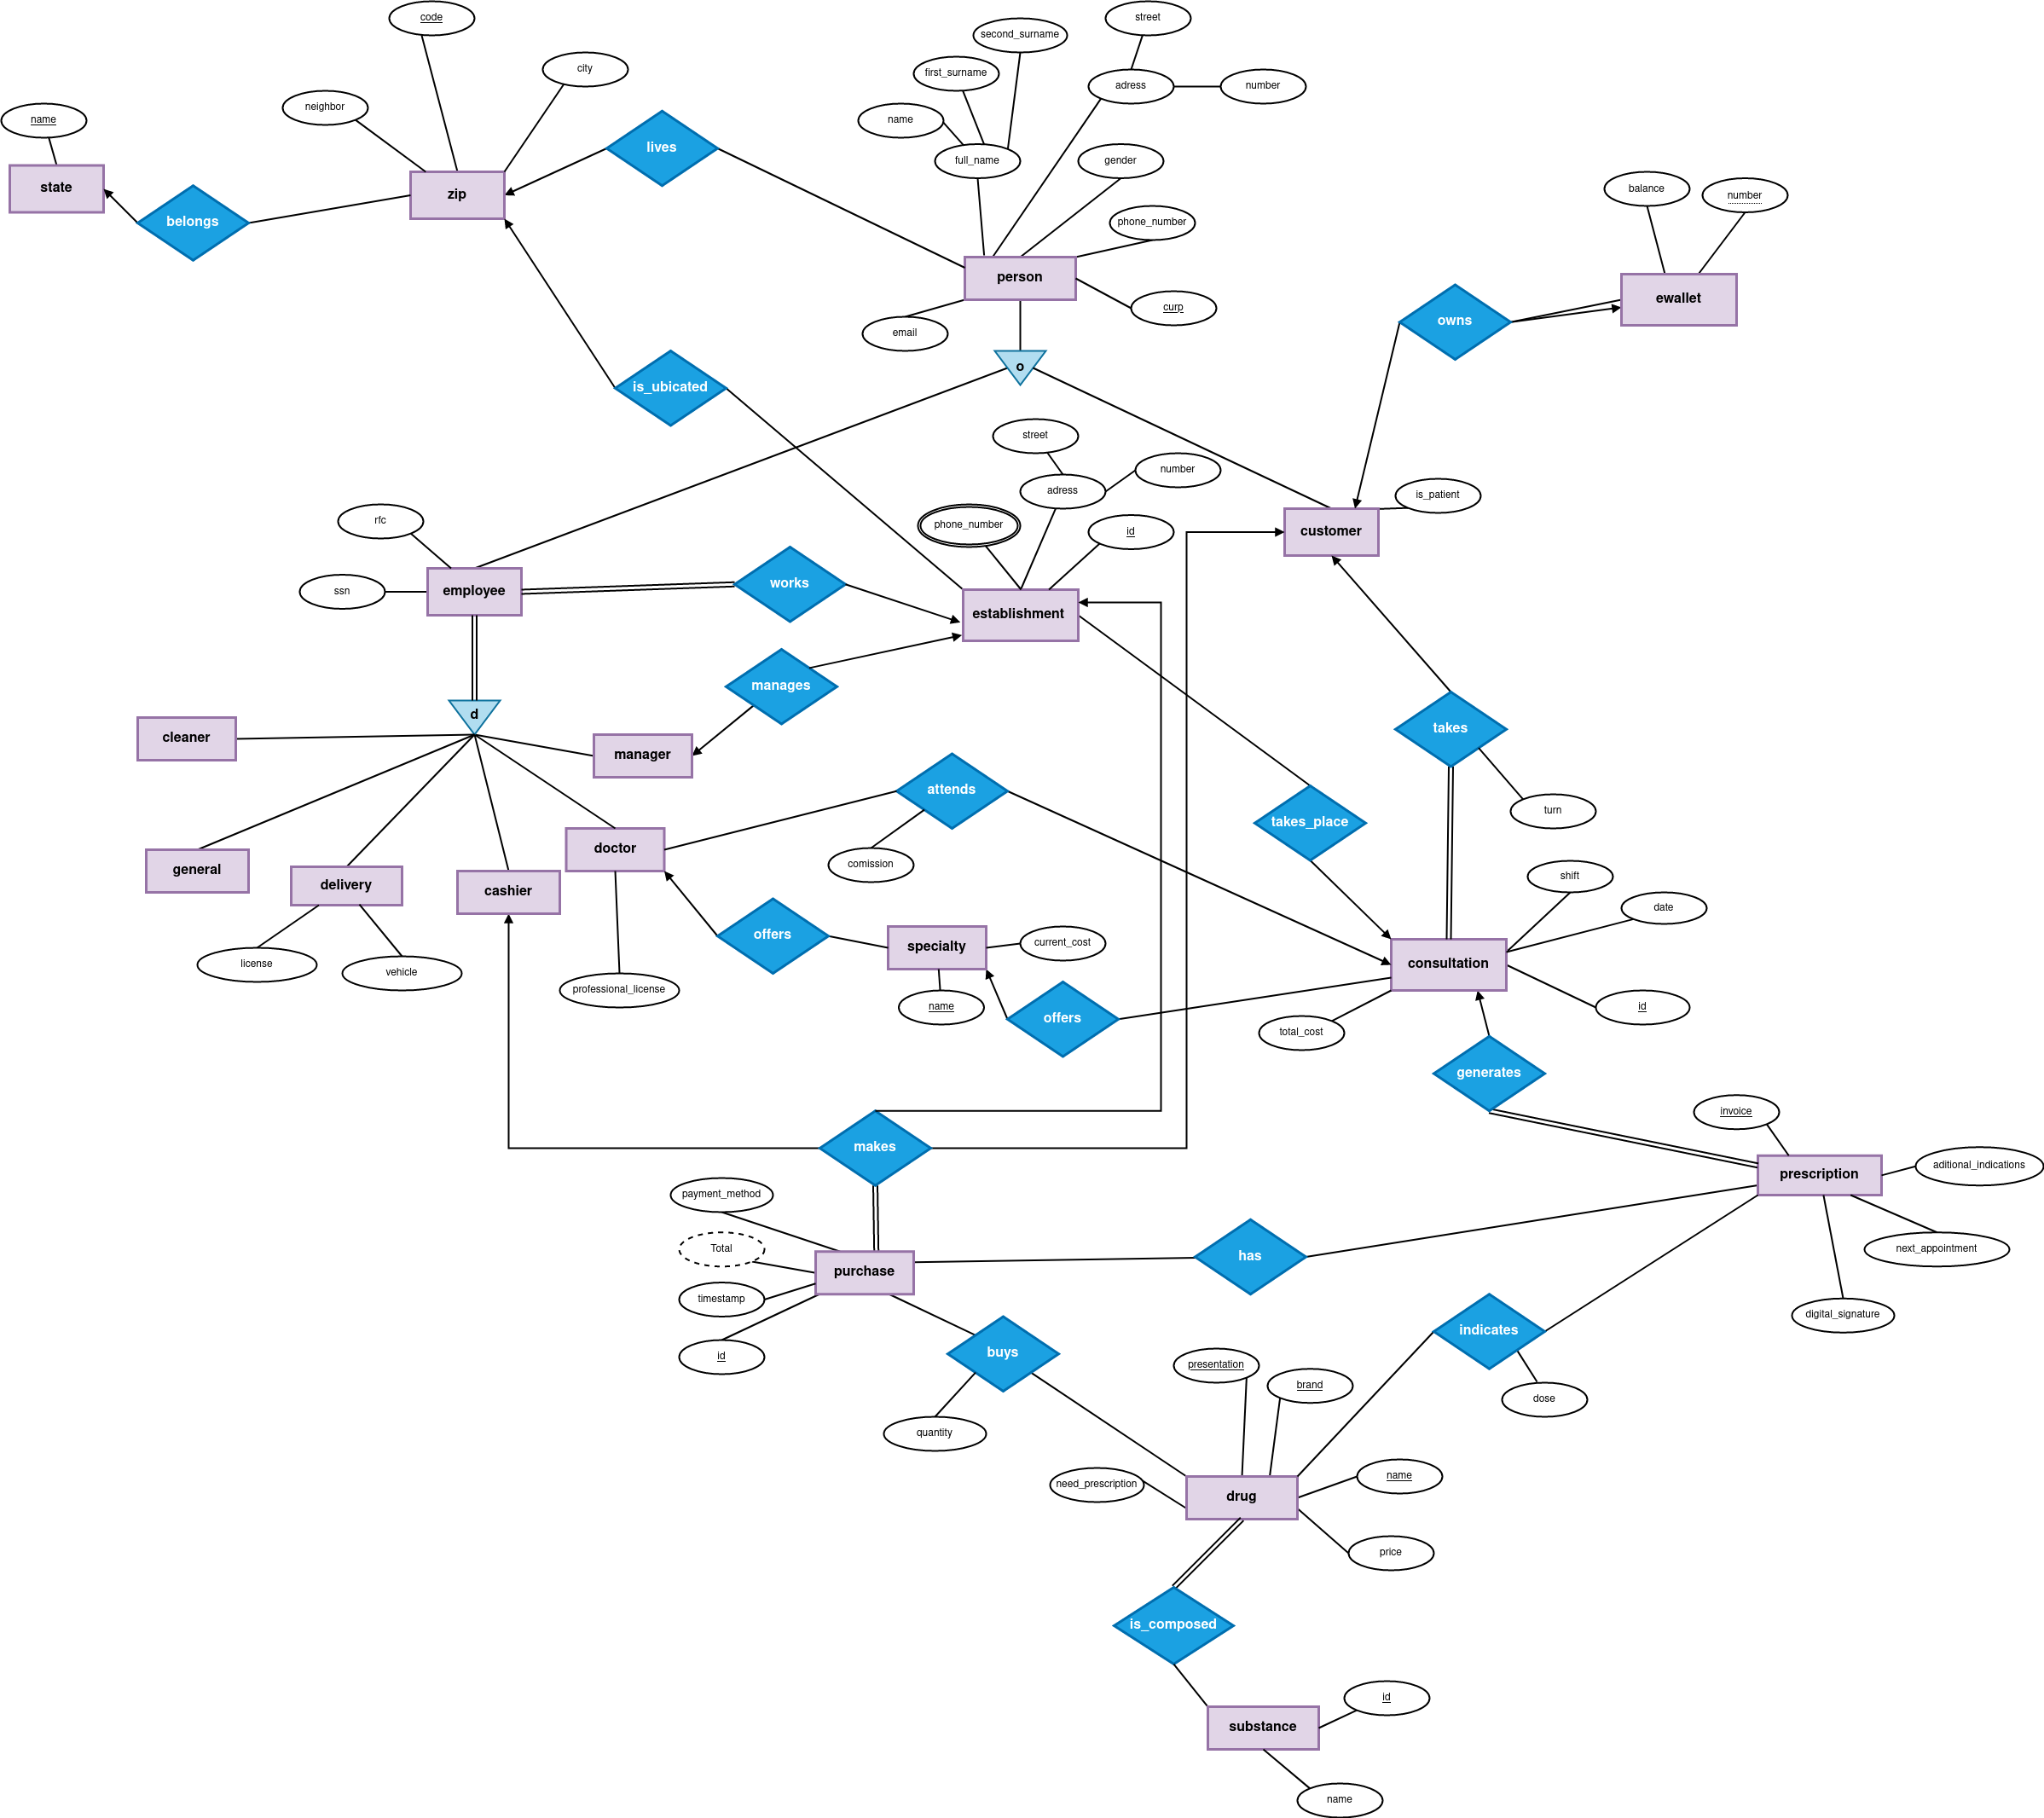
\includegraphics[width=\textwidth]{Entidad_Relacion}
        \end{figure}


    % ======================================================================================
    % =====================           MODELO RELACIONAL           ==========================
    % ======================================================================================
    \chapter{
       Modelo Relacional y los requerimientos}

      % =====================================================
      % ============           ENTIDADES             ========
      % =====================================================
      \section{Relaciones creadas}

        Algo importante a destacar es que en esta sección solo hablaremos de manera general sobre el proceso de transformación entre
        el modelo entidad relación extendido y el modelo relaciónal, no daremos una visión detallada y explicación de cada una de las 
        relaciónes resultantes, si se necesita consultar dicha información le indicamos que el mejor lugar es el diccionario de datos
        donde podrá saber más sobre los mismos.

        \subsection{Sobre personas y empleados}

            De manera análoga a lo que hicimos, para el modelo entidad 
            relación empecemos con la entidad \texttt{person}, pasarla al modelo relaciónal es trivial siguiendo las pautas que conocemos del curso
            eliminamos atributos compuestos (name) y ponemos los \Quote{atributos hoja}, y como llave foránea colocamos la llave primaria de la 
            relación \texttt{zip}, este también fue sencillo de pasar al modelo relaciónal se eliminaron las relaciónes intermedias en vez de eso
            como vimos en clase se agregó una llave foránea que sea la llave primaria de la relación \texttt{state}.

            \texttt{person} no desaparece pues su especialización no es total, es decir en esta solución que estamos proponiendo existe 
            la posibilidad de tener personas que sean doctores y clientes al mismo tiempo o empleados generales que también sean repartidores.

            La entidad que si tenía una especialización total fue \texttt{employee} que desaparece y los atributos son absorbidos por
            sus entidades hijas. En este caso estas son \texttt{general} (que tiene el identificador del establecimiento como llave
            foránea, el rfc y el numero de seguridad social), de manera idéntica con \texttt{cleaner}, \texttt{manager}, \texttt{cashier},
            y de manera parecida con \texttt{deliveryman} (agregando sus atributos únicos), \texttt{doctor} (agregando sus atributos únicos).

        \subsection{Sobre establecimientos, los medicamentos y consultas}

            Creamos la relación \texttt{establishment}, de manera parecida a \texttt{person} contiene un atributo que es una llave foránea 
            a la relación \texttt{zip}.
            Otro  interesante es la creación de \texttt{phone\_number} una relación que ahora nos permite tener varios números de teléfono asociados
            a un establecimiento.

            Ahora hablemos de las medicinas, la entidad \texttt{drug} es igualmente fácil de traducir usando las reglas que vimos en la clase,
            ahora si conservamos la relación \texttt{buys} que básicamente contiene las llaves primarias de \texttt{purchase} y \texttt{drug}
            y la cantidad, de manera análoga con la anterior relación \texttt{is\_composed} y con \texttt{indicates}.

      % =====================================================
      % ============           DIAGRAMA              ========
      % =====================================================
      \section{Diagrama final}

        \begin{figure}[ht]
            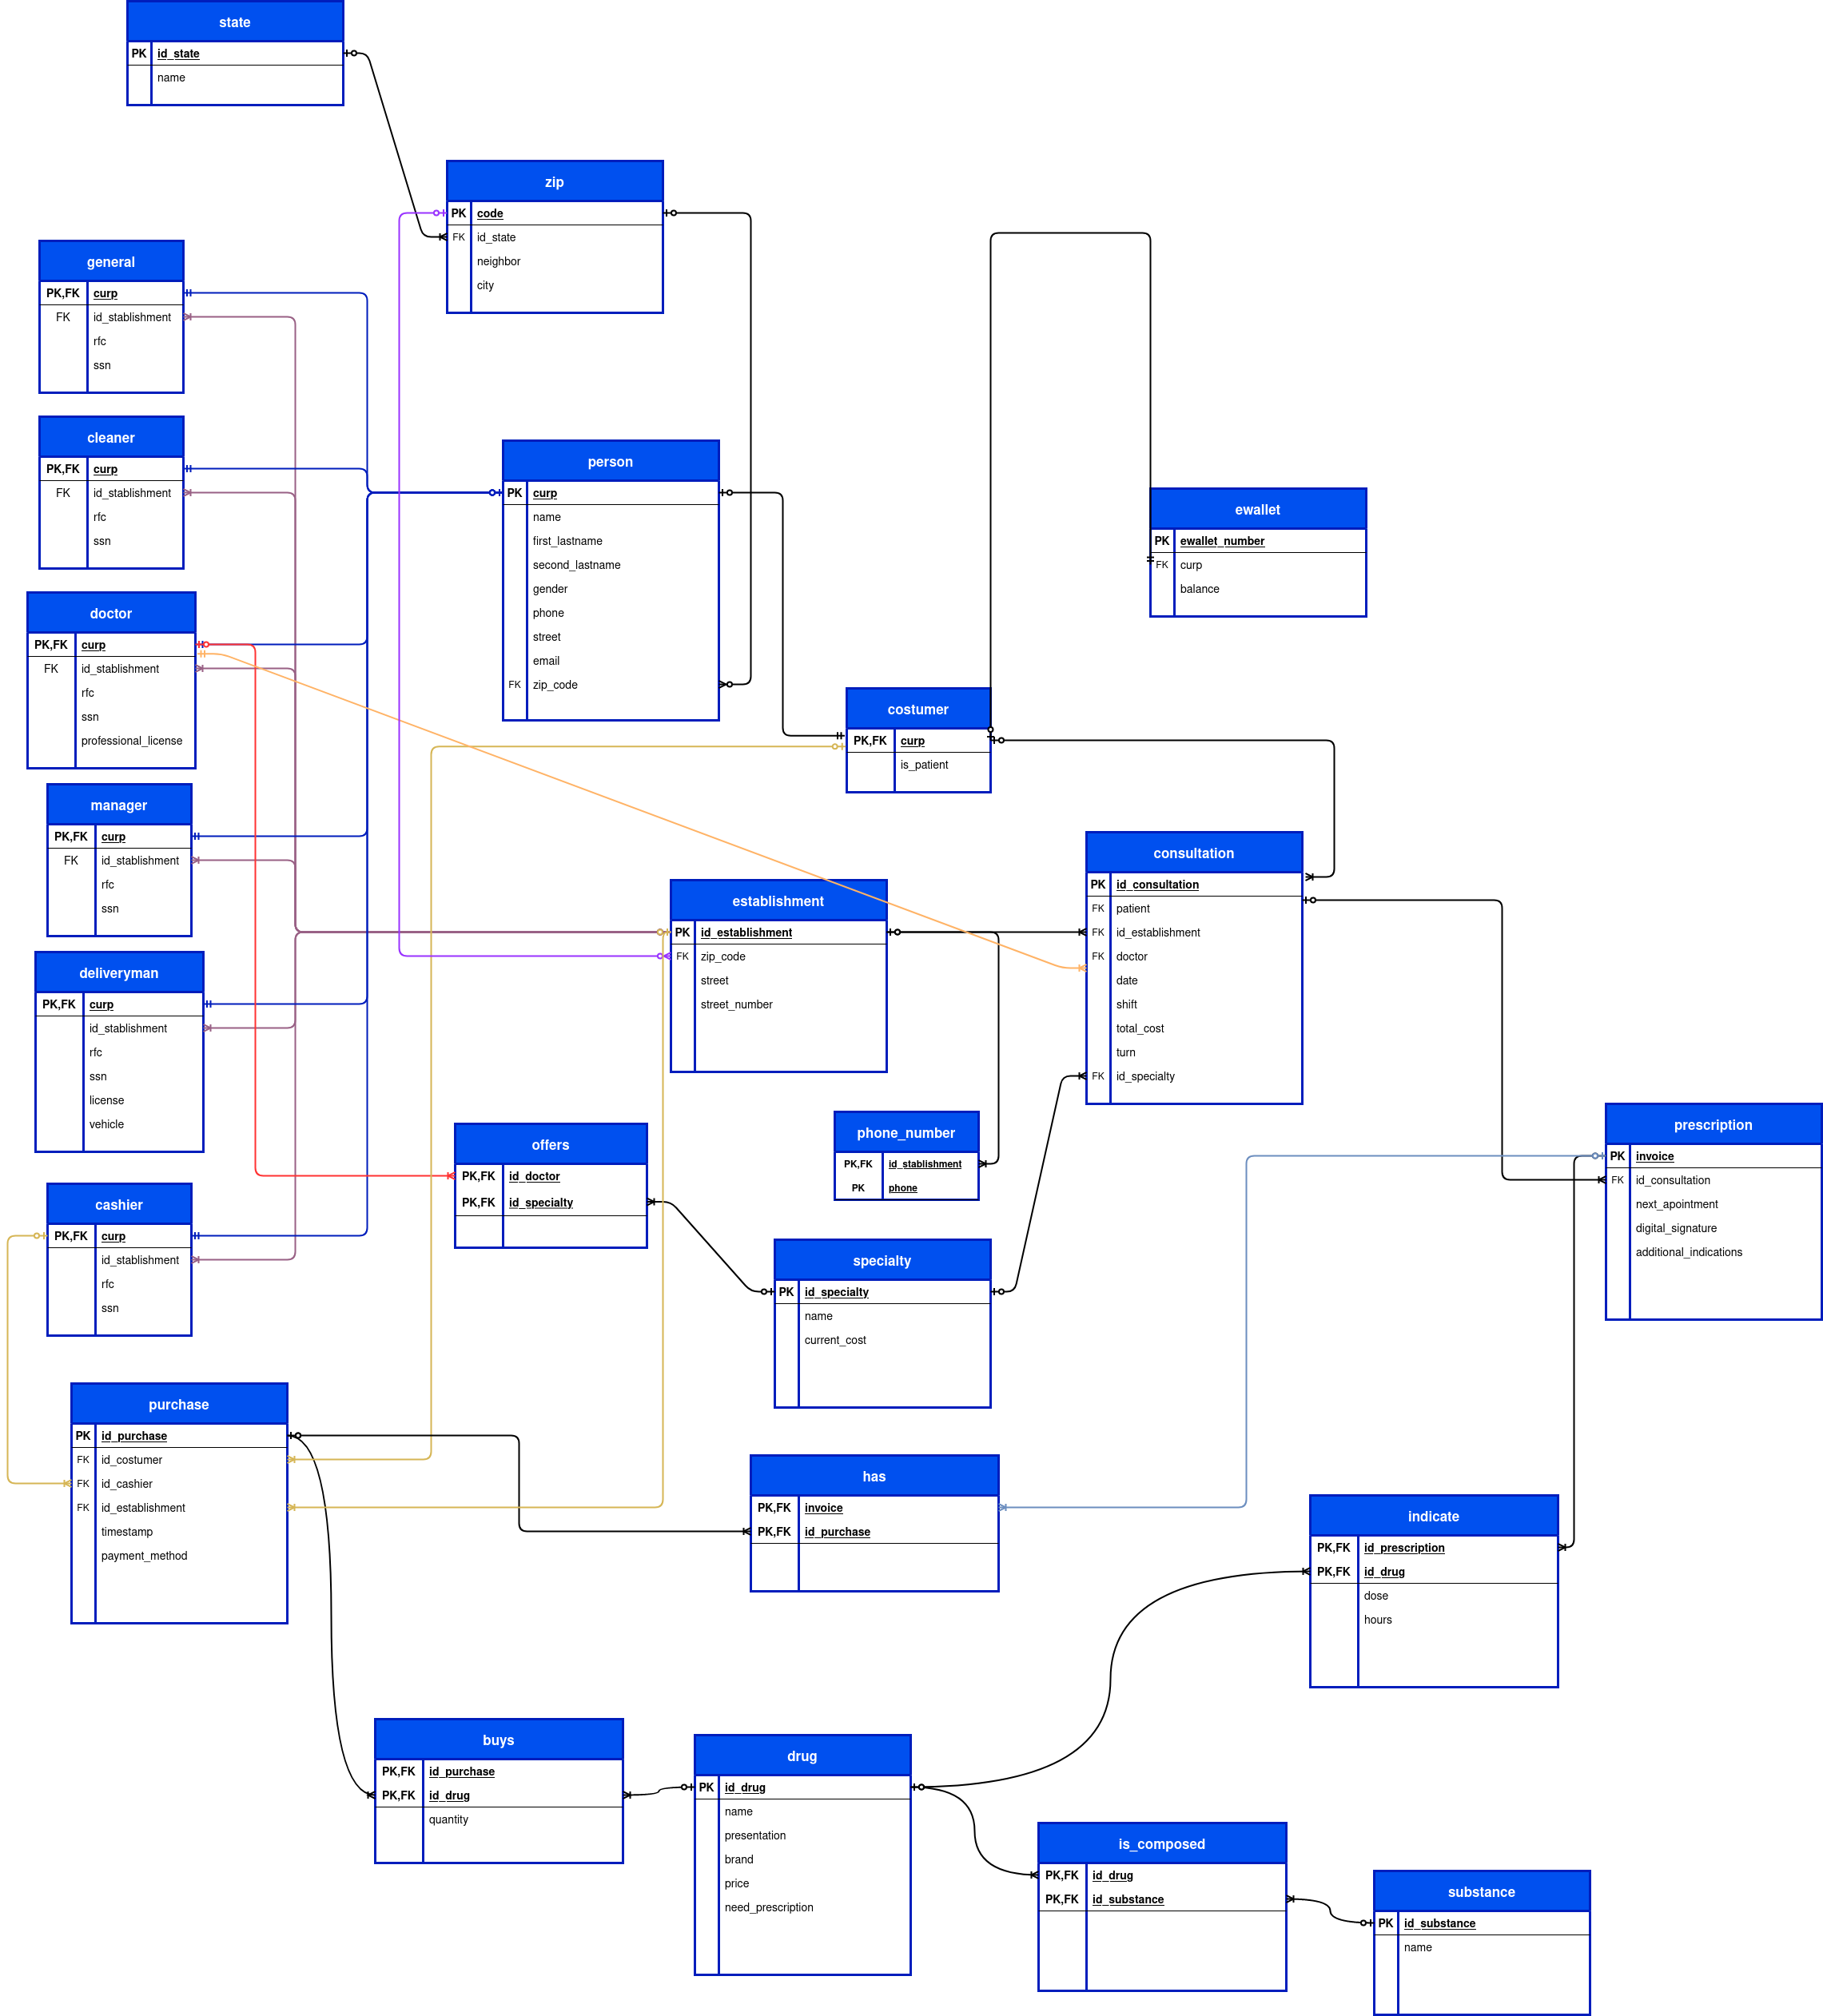
\includegraphics[width=0.7\textwidth]{Relacional}
        \end{figure}

    % ======================================================================================
    % =====================                 NORMALIZACION           ========================
    % ======================================================================================
    \chapter{Normalización}

    \section{¿Que es la normalización?}

        Una relación bien estructurada.

        Es aquella que permite libremente escribir, actualizar o eliminar un registro sin que
        ocurran anomalías.

        En otras palabras una relación bien estructurada, es aquella relación que contiene el
        mínimo de redundancia y permite a los usuarios insertar, modificar y borrar registros
        en una tabla sin errores o inconsistencias.

    \subsection{Definición}

        Decimos que normalizar es el proceso por el cual convertimos todas nuestras relaciones
        en relaciones bien estructuradas y pequeñas.
        Es decir, a efectos prácticos lo que hacemos es dividir las relaciones que tenemos.

        Podemos decir alternante que Normalización es el proceso de eliminación de
        redundancias en una tabla para que sea más fácil de modificar.

        Podemos decir que la normalización es de descomposición de las tablas para eliminar
        información redundante y anomalías al momento de insertar, actualizar o eliminar la
        información.


      % =====================================================
      % ============           1FN                   ========
      % =====================================================
      \section{Primera Forma Normal}

        Llegar a primera forma es muy sencillo, sobretodo considerando el proceso 
        que ya llevamos hasta llegar aquí.

        Basta con asegurarnos que cada atributo sea atómico, es decir eliminar los atributos multivalor ...
        y podemos decir que no tenemos atributo multivalor, en nuestro diagrama solo tenemos un solo atributo multivaluado
        que fue correctamente traducido a una relación extra lo cual nos permite que el atributo teléfono siga siendo atómico.

        De los demás atributos podemos decir que todos son claramente atómicos con unas contadas casi excepciones:
        \begin{itemize}
            \item \texttt{name} no es atómico si consideramos a personas con dos nombres, pero dado que solo vamos a ocupar el nombre para 
            mostrarlo y en ese caso siempre acabaremos concatenando ambos nombres podemos considerar al conjunto de todos los nombres
            que tenga una persona como tóxicos para nuestro caso.
            \item \texttt{additional\_indications} este será un campo de texto y es bastante posible que el texto sea una serie de indicaciones
            por ejemplo: \Quote{reposo, no comer comida picante y evitar la actividad física intensa por 3 dias}, y si desde un punto de vista
            semántico podemos discutir que estos son en realidad 3 indicaciones, pero es que de igual manera no tiene sentido mucho separarlas 
            sobretodo considerando que al ser personas diferentes podemos acabar con indicaciones muy parecidas pero que no son iguales como
            evitar salir a correr por 3 dias y no hacer actividad fisica en 3 días, lo cual nos causaría una enorme cantidad de problemas y de 
            la misma manera este campo solo será usado para ser mostrado al doctor que haga la próxima consulta y seguimiento, por lo que para
            esta solución de igual manera consideramos que las indicaciones son atómicas.
        \end{itemize}


      % =====================================================
      % ============           2FN                   ========
      % =====================================================
      \section{Segunda Forma Normal}

        \subsection{Dependencia Funcional y Determinantes}

            Al hablar de la normalización tenemos que hablar casi obligatoriamente
            de dependencias funcionales y de los determinantes.

            Decimos que una dependencia funcional es una restricción entre dos conjuntos
            de atributos en la base de datos.

            Es decir, en una relación $R(Atributo_1, Atributo_2, \dots)$ sean $X$ y $Y$ subconjuntos de $R$, de la forma: $X = \{Atributo_a, Atributo_b, \dots\}$ y 
            $Y = \{Atributo_\alpha, Atributo_\beta, \dots\}$ entonces decimos que:

            \textbf{Hay una dependencia funcional de $X$ a $Y$ denotada por $X \lLongTo Y$
            si y sólo si es que para cualquiera dos tupla $t_1, t_2$ de nuestra base de
            datos, si los valores de $t_1$ son iguales a los de $t_2$ en X, entonces
            también su valores serán iguales en los atributos de $Y$}.

            \textbf{Decimos por lo mismo que $X$ determina a $Y$, por eso es común ver que se llama
            a $X$ como el determinante de una dependencia funcional}.


        \subsection{Definicción}

            Antes, antes, antes, para hablar de la segunda forma normal tenemos que 
            hablar de lo que es una dependencia funcional parcial y total:

            \begin{itemize}
                \item \textbf{Dependencia Funcional Parcial:}

                    Decimos que tenemos una dependencia funcional parcial $X \lLongTo Y$
                    si es que podemos encontrar encontrar un subconjunto de $X$ que también
                    determina a $Y$.

                \item \textbf{Dependencia Funcional Total:}

                    Decimos que tenemos una dependencia funcional total $X \lLongTo Y$
                    si es que NO podemos encontrar encontrar un subconjunto de $X$ que también
                    determina a $Y$.
            \end{itemize}

            Decimos que una Relación $R$ esta en su segunda forma normal
            si y solo sí todos los atributos que no son llaves primarias, secundarias
            o candidatas solo dependen de la llave primaria.

            O de otro modo decimos que un esquema de relación $R$ está en 2FN si
            todo atributo no primo depende funcionalmente de manera total de la
            clave primaria de R.

        \subsection{Nuestro caso}

            Ahora vayamos relación a relación para ver que no hay una sola que no cumpla la segunda forma normal, recordemos que la segunda
            forma normal se puede resumir como \Quote{the hole key}.

            \begin{itemize}
                \item para \texttt{state} solo tenemos un atributo por lo que es trivial que se cumplea 2FN
                \item para \texttt{zip} es igualmente sencillo porque solo tenemos una llave, es decir no poder hacer conjuntos propios no
                vacíos a partir de ella.
                \item para \texttt{specialty} igual, 1 llave, es decir no poder hacer conjuntos propios no vacíos.
                \item para \texttt{drug} igual, 1 llave, es decir no poder hacer conjuntos propios no vacíos.
                \item $\cdots$, para evitarnos repetir las 24 relaciones solo hablaremos de aquellas que tengan más de un atributo como
                llave primaria.
                \item nota que para casos como \texttt{phone\_number} es cierto que tenemos una llave compuesta, pero es que no tenemos
                nada mas que llaves, no hay atributos no primos, por lo que es imposible incumplir la 2NF.
            \end{itemize}

            y bueno, hemos acabado todas las relaciones que tenemos, por lo que es trivial hablar de que nuestra solución ya esta
            en 2NF.


      % =====================================================
      % ============           3FN                   ========
      % =====================================================
      \section{Tercera Forma Normal}
     
        \subsection{Nuestro caso}
            Este se base en el concepto de dependencia transitiva.
            Una dependencia funcional $X \lLongTo Y$ en un esquema de relación $R$
            es una dependencia transitiva si existe un conjunto de atributos $Z$
            que no sea subconjunto de las llaves claves de $R$, y se cumplen
            que si $X \lLongTo Y$ como $Y \lLongTo Z$, entonces $X \lLongTo Z$.

            En la 3FN se elimina las dependencias transitivas; es decir atributos no
            clave no dependen de otros atributos no clave.

            Decimos que una Relación $R$ esta en su segunda forma normal
            si y solo sí todos los atributos solo dependen de la llave primaria. 

            Es decir, tenemos que asegurarnos que todo atributo no dependa de nada mas que de la llave:

        \subsection{Nuestro caso}

            \begin{itemize}
                \item Hay tablas triviales como \texttt{is\_composed} en las que como 
                    no tenemos atributos que sean llave es trivial que se cumple 3FN
                \item Hay tablas triviales como \texttt{state}, \texttt{substance}, 
                \texttt{offer}, 
                \texttt{phone\_number}, 
                \texttt{customer}, 
                \texttt{has}
                 en las que como 
                    solo tenemos un atributo es trivial que se cumple 3FN
                \item para \texttt{zip} todo depende solo de la llave, se cumple 3FN
                \item para \texttt{specialty} igual, del id depende el nombre y con el nombre no podemos saber el costo
                ni inversamente.
                \item para \texttt{drug} podriamos argumentar que dado el nombre podriamos deducir la marca pero eso 
                no se puede aplicar para todos los casos (solo en medicamentos de patente, que por el giro del negocio
                seran minimos).

                Ademas otro dependencia interesante es que si usamos el nombre, la marca y la presentacion entonces 
                podemos acotar el precio, y si, tecnicamente eso incumple la 3FN lo que nos dictaria usar la tupla
                nombre, marca y presentación como llave primaria compuesta, pero esto traería dos problemas, primero que
                nada en el rendimiento pues usar esos 3 valores como llave primaria haria inecesariamente lento usar la tabla y
                que ahora usar estas como llaves foraneas complicaria bastante su uso, por esto decidimos ignorar esta dependecia funcional
                y elegir un id como llave para esta tabla.

                \item para \texttt{doctor} podriamos argumentar dado el turno podriamos adivinar y la fecha podriamos adivinar el doctor pero
                en nuestra solucion el responsable de un turno es solo eso, el responsable, es decir no hay impedimento para que algun otro doctor 
                haga una consulta sin ser el responsable, esta es la unica posible dependencia transitiva que incumpliria la 3FN, 

                \item para \texttt{purchase} podriamos argumentar que el total deberia ser un atributo calculado y no estar presente, pero es que debido
                a los programas de cliente frecuente de la sucursal el total de una compra puede ser menor que la suma de cada una de los elementos comprados
                y como las compras una vez creadas son inmutables para nuestra solucion entonces es necesario tener ese atributo.

                
                \item para \texttt{establishment}, 
                \texttt{person},
                \texttt{ewallet},
                \texttt{doctor},
                \texttt{deliveryman},
                \texttt{prescription},
                \texttt{indicates},
                \texttt{general},
                \texttt{buys},
                \texttt{cleaner},
                \texttt{cashier}
                consideramos que no hay ambigüeadad y es obvio que no existe dependencia funcional transitiva que incumpla la 3NF
            \end{itemize}


    % ======================================================================================
    % =====================         IMPLEMENTACION EN SQL           ========================
    % ======================================================================================
    \chapter{Implementación es SQL}

        Nosotros usamos PostreSQL para nuestra implementación, en la carpeta adjunta a este reporte agregamos varios documentos, nota
        importante es que usamos tanto en el \texttt{ddl.sql} como en \texttt{poblamiento.sql} una transaccion para evitar dejar a nuestra base
        de datos en un estado inconsistente si existiera algun fallo.

        \section{DDL}

            Contiene el codigo necesario para crear las tablas y enums que usamos para nuestra solucion estos mismos basados en el modelo
            relacional que hablamos en la seccion anterior.

        \section{Población de datos para pruebas}

            Contiene el codigo necesario para poblar con datos \Quote{dummy} y podamos probar nuestra solución mas adelante

        \section{Triggers}

            Hablaremos de los posibles trigger y constraints que serian necesarios en nuestra solucion para garantizar una consistencia de datos.
            \begin{itemize}
                \item Un trigger que nos asegure que al momento de crear una nueva sucursal esta ya tiene que tener asociada un cliente
                por defecto y que dicho cliente tiene que cumplir con ciertas caracteristicas (como un nombre que nos indique la farmacia o que no tenga
                ewallet).

                \item Un trigger que nos ayude a mantener el control de als consultas gratuitas, este correra al momento de intentar agregar una nueva tupla
                a la tabla donde guardamos las consultas gratuitas, y se asegurara que es valida, es decir que la consulta fue general y que para en dia dado en cierta
                sucursal no existen mas de otras 4 consultas gratis.

                \item Un trigger que corra al momento despues de realizarse una compra, en este veremos el tipo de pago, si fue co ewallet le hacemos un descuento all ticket por
                ell 5\%, de ser de un cliente con ewallet agregamos un 3\% del total a su balance.

                \item Un trigger al momento de realizar una consulta, donde verifiquemos que si dicha persona aun no estaba registrada como paciente entonces
                la agregamos, y relacionado con el mismo uno que nos impida actualizar dicho valor dentro de la tabla cliente para cambiar de paciente a no
                paciente.

            \end{itemize}


        \section{Funciones}

            Un archivo llamado \texttt{extra.sql} donde tenemos un stored procedure que nos permite cambiar de manera atomica
            (mediante transacciones) cambiar el manager responsable de cierta sucursal y tambien una funcion auxiliar que nos permite
            saber si es posible que un cliente dado pueda comprar un medicamento considerando si tiene receta y si la dosis es la que esta
            escrita (o menor si va a hacer varias compras).



% ////////////////////////////////////////////////////////////////////////////////////////////////////////////////////
% ////////////////////////////////////////   QUERIES DEL SISTEMA     /////////////////////////////////////////////////
% ////////////////////////////////////////////////////////////////////////////////////////////////////////////////////
\part{Demostración de nuestra solución}

    % ======================================================================================
    % =====================              QUERIES                  ==========================
    % ======================================================================================
    \chapter{Queries}

        
        \section{Comparemos ventas por sucursal}
            
            \begin{figure}[ht]
                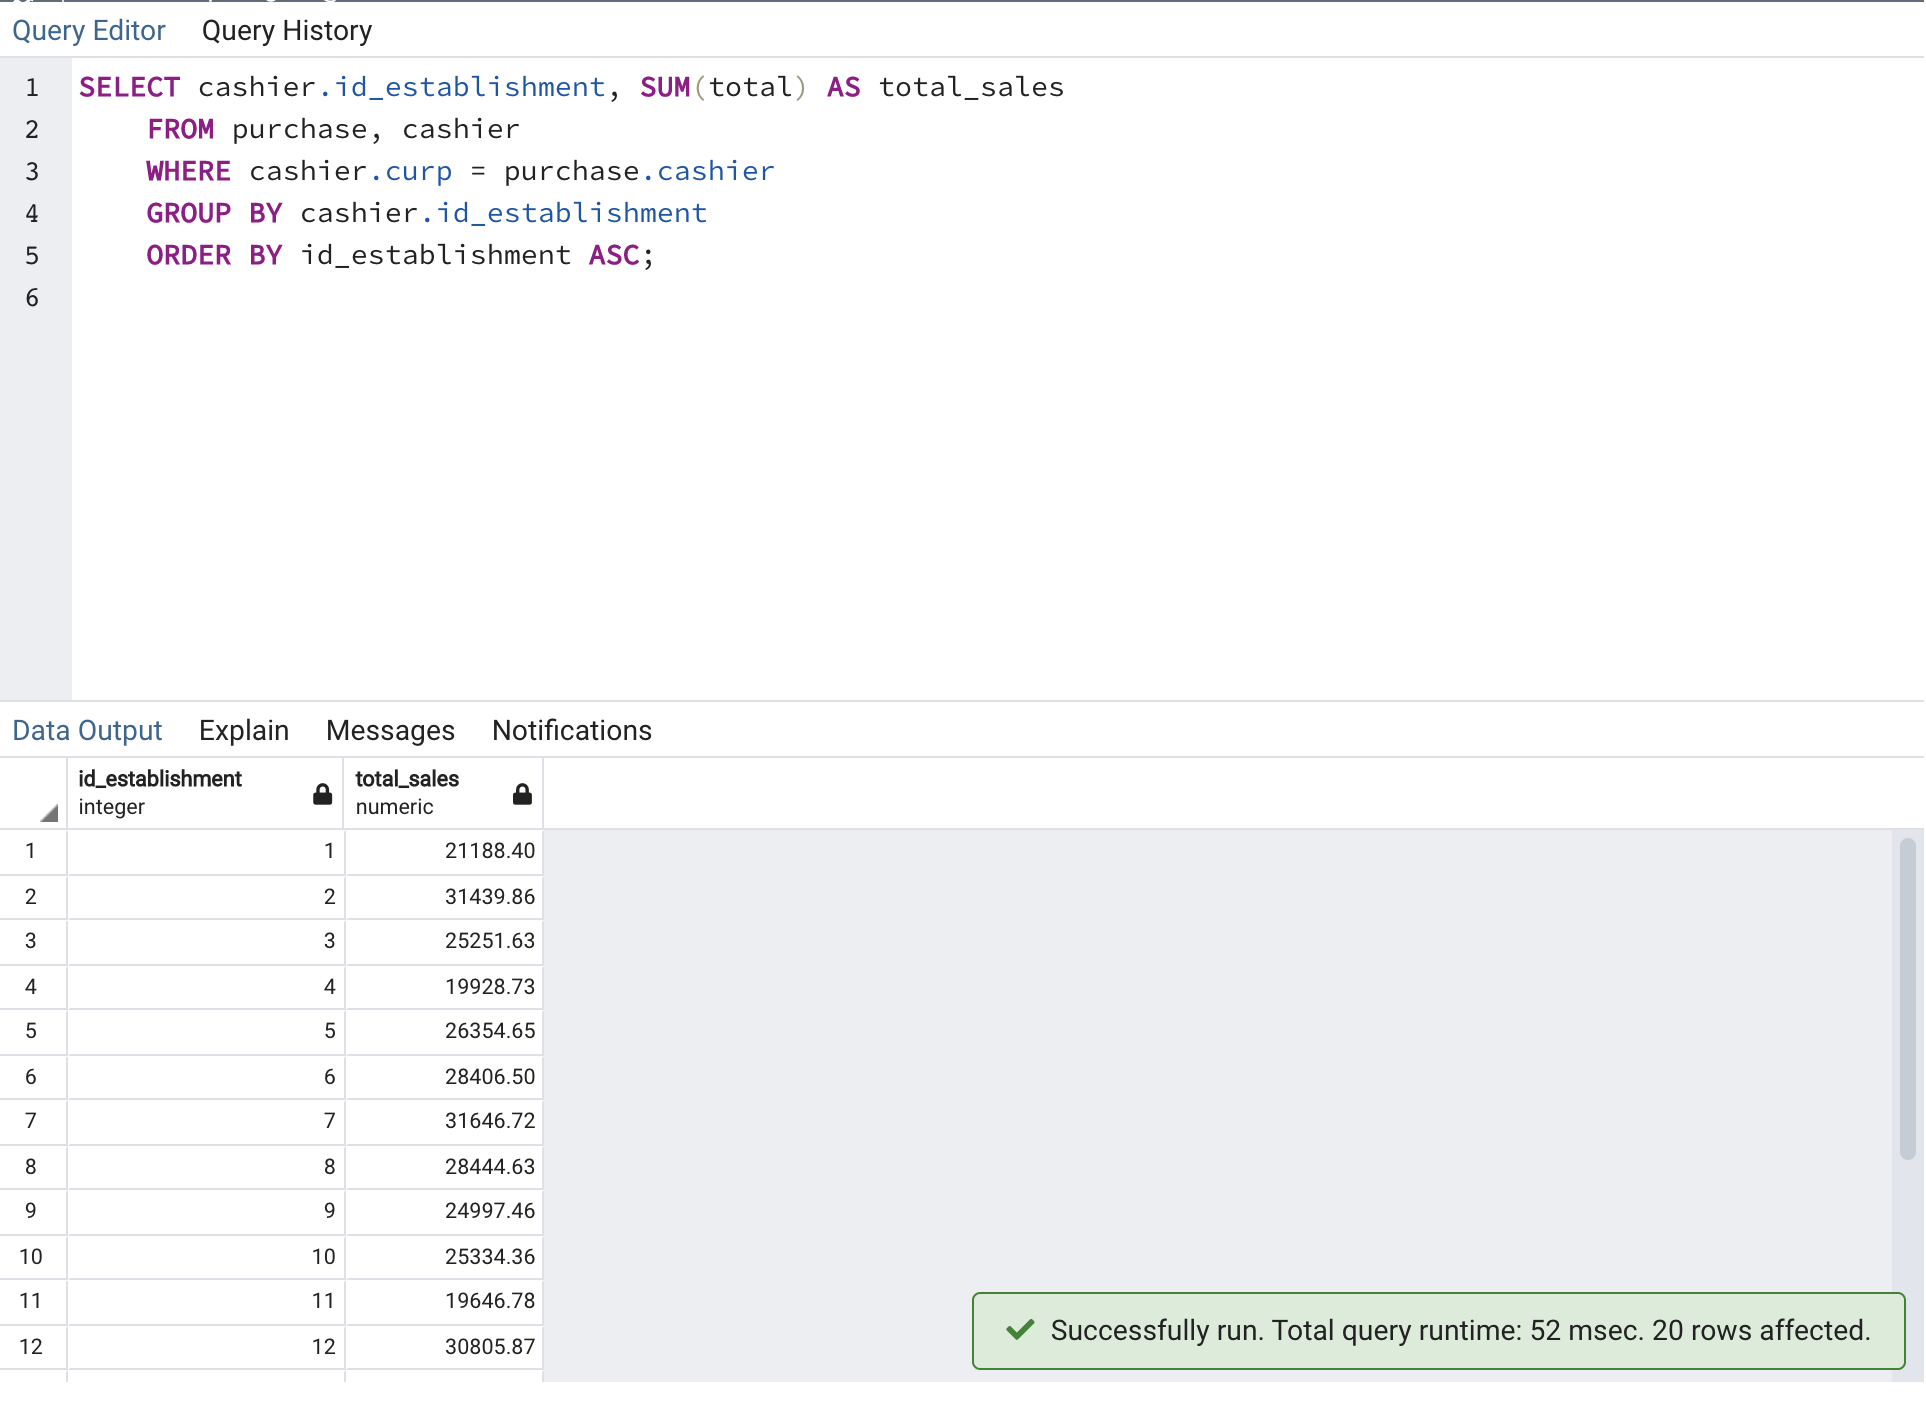
\includegraphics[width=0.9\textwidth]{1}
                \caption{Con nuestra solución podemos hacer consultas para comparar con información a 
                tiempo real las ventas de cada sucursal y ordernarlas por sucural}
            \end{figure}

        \clearpage
        \section{Número de consultas por doctor}
            
            \begin{figure}[ht]
                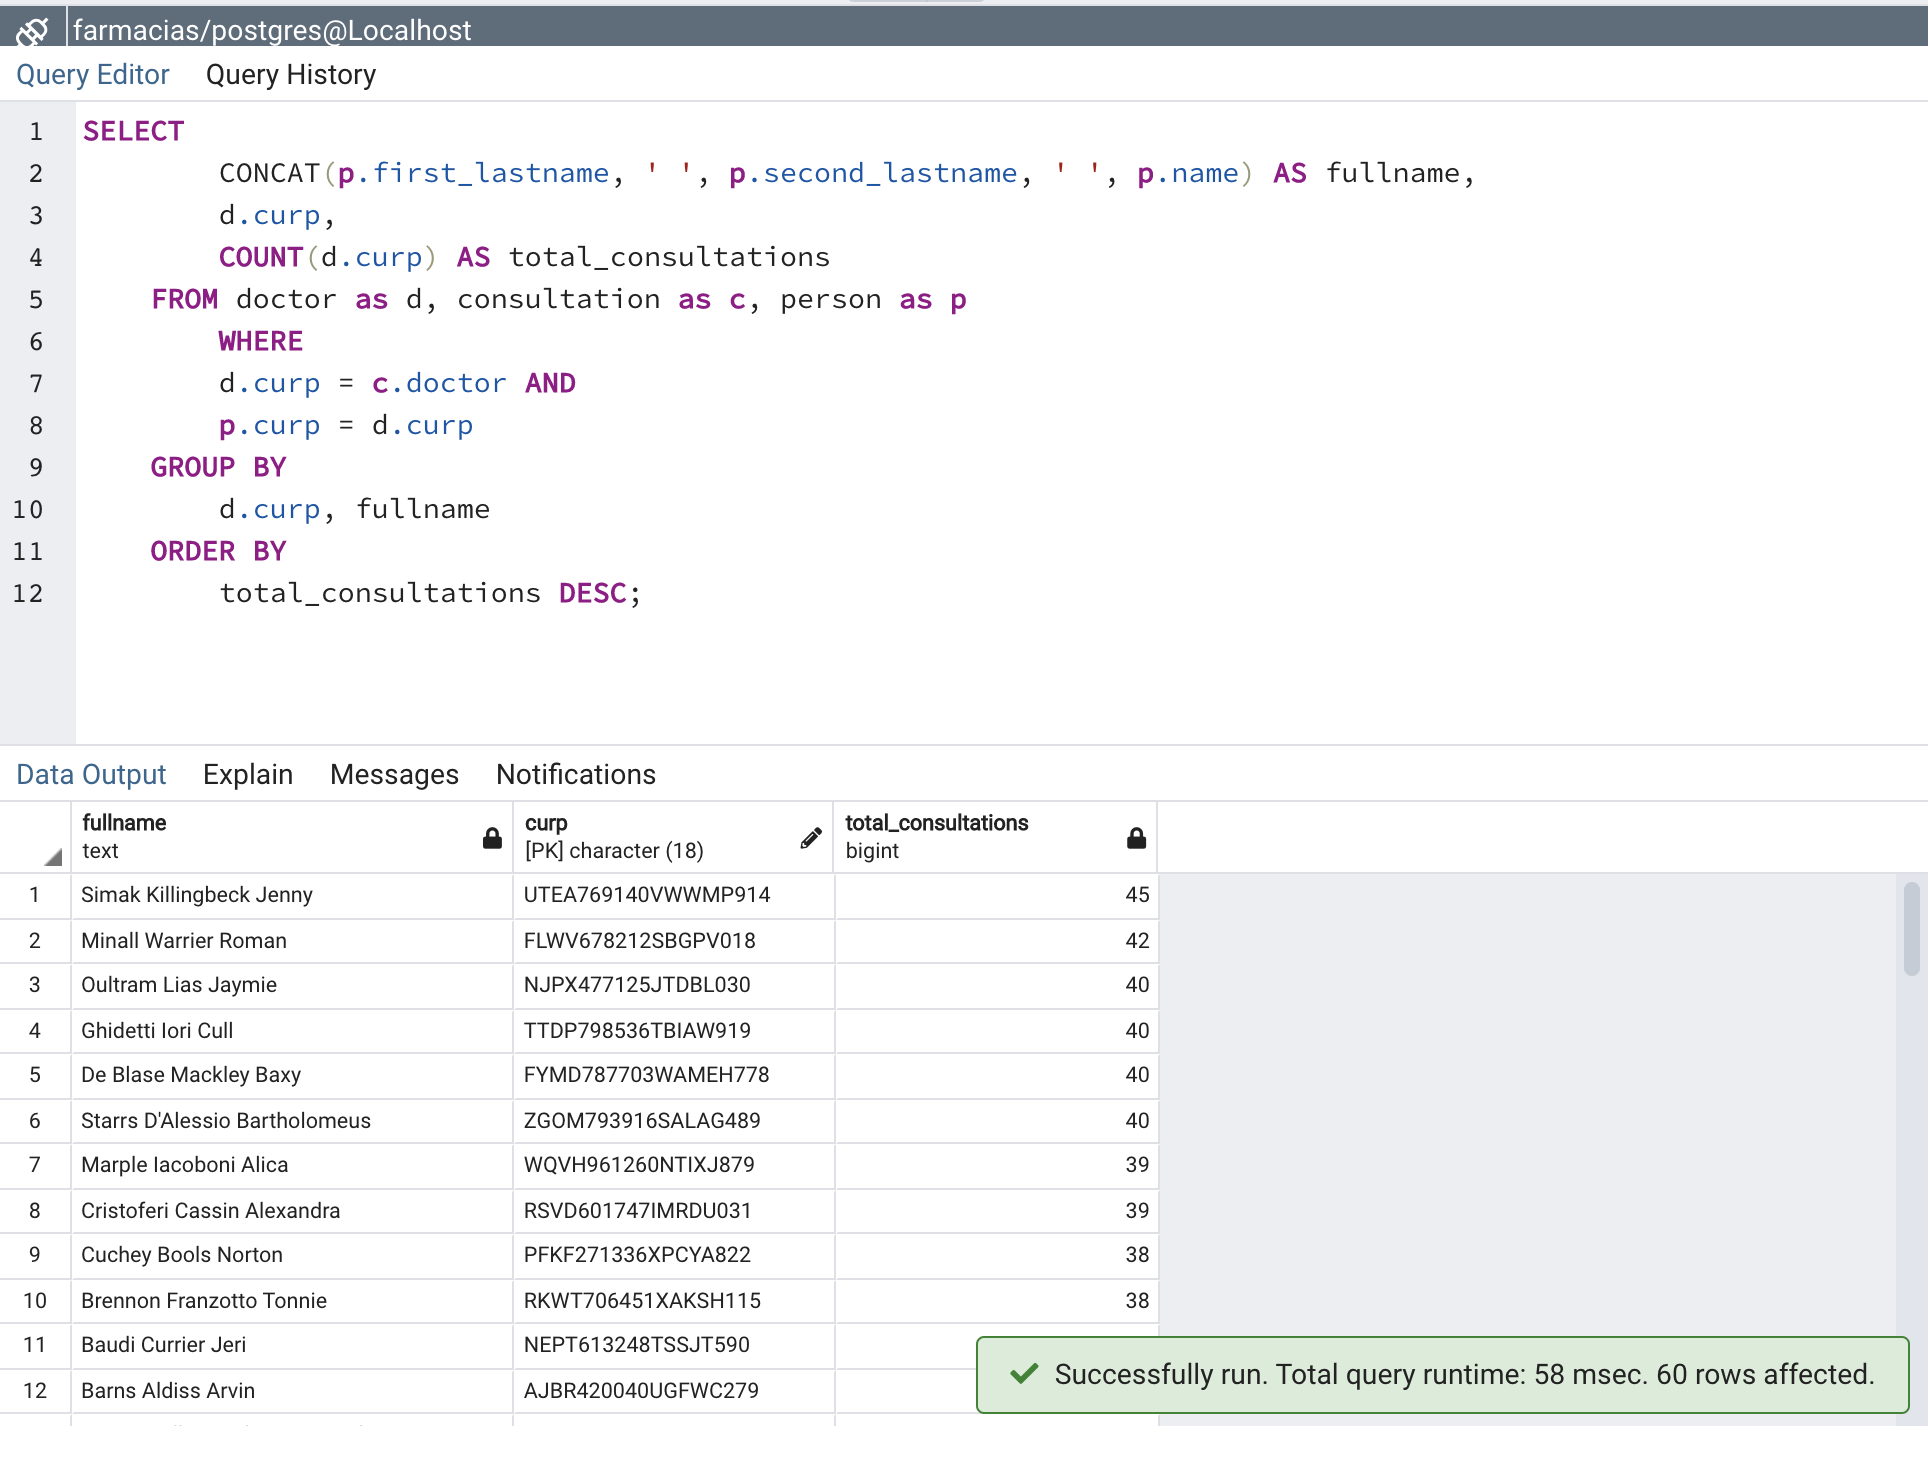
\includegraphics[width=0.9\textwidth]{2}
                \caption{Con nuestra solución podemos medir la productividad de cada doctor mostrando las
                consultas que han dado y ordernadolos por de mayor a menor usando dicha metrica}
            \end{figure}

        \clearpage
        \section{Número de consultas por mes del año}
            
            \begin{figure}[ht]
                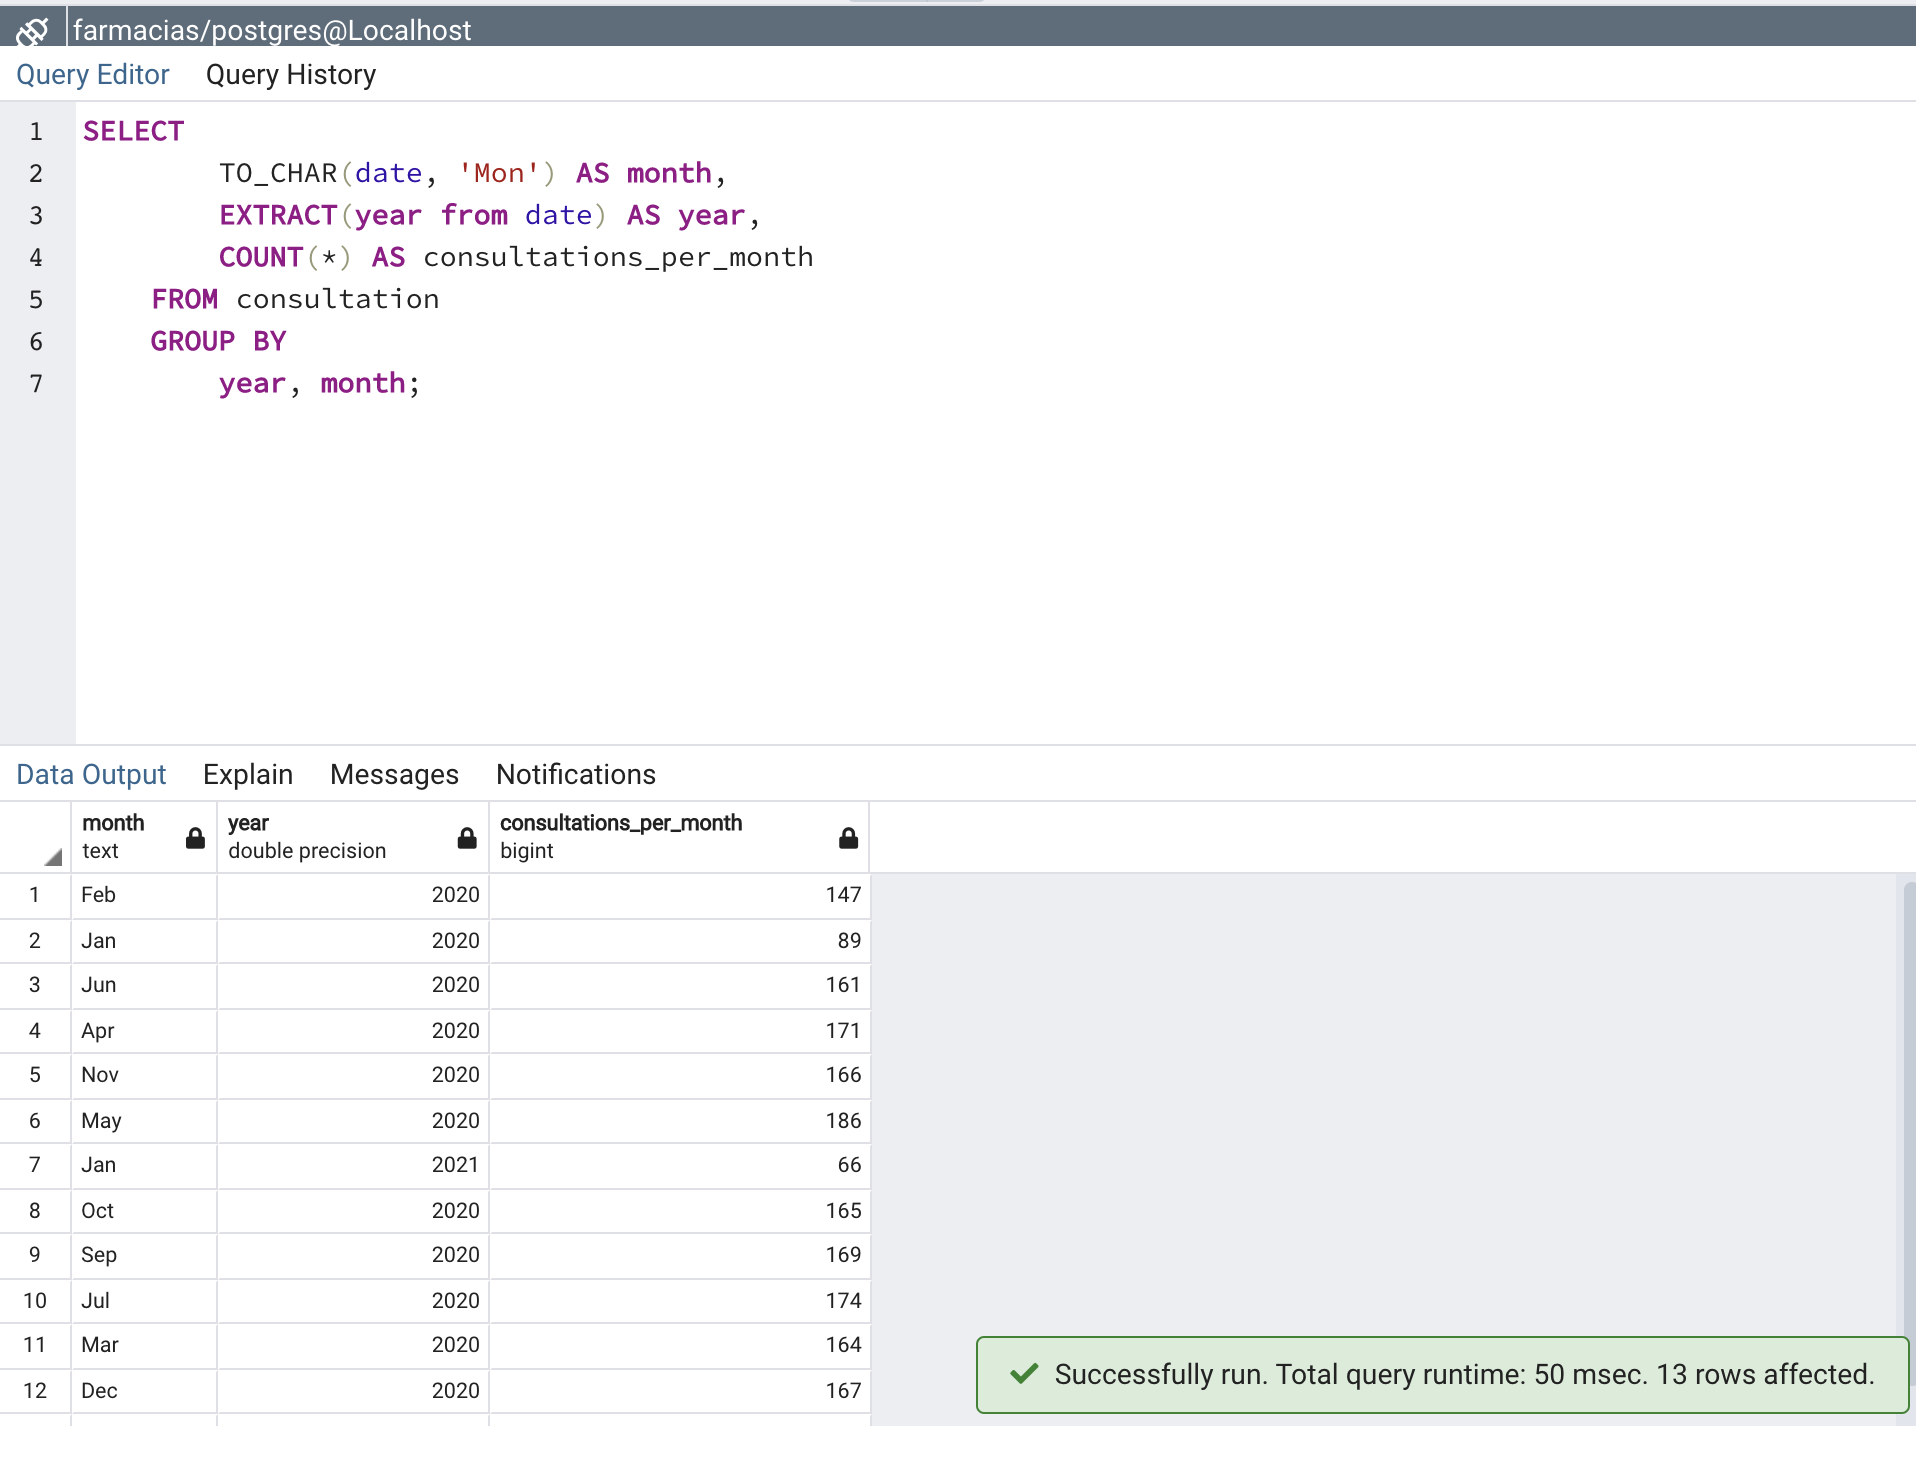
\includegraphics[width=0.9\textwidth]{3}
                \caption{Con nuestra solución podemos tambien ver las fluctuaciones a lo largo del año en el
                numero de consultas creadas, permitiedo alocar de mejor manera recursos con esta información}
            \end{figure}

        \clearpage
        \section{Productos más vendidos}
            
            \begin{figure}[ht]
                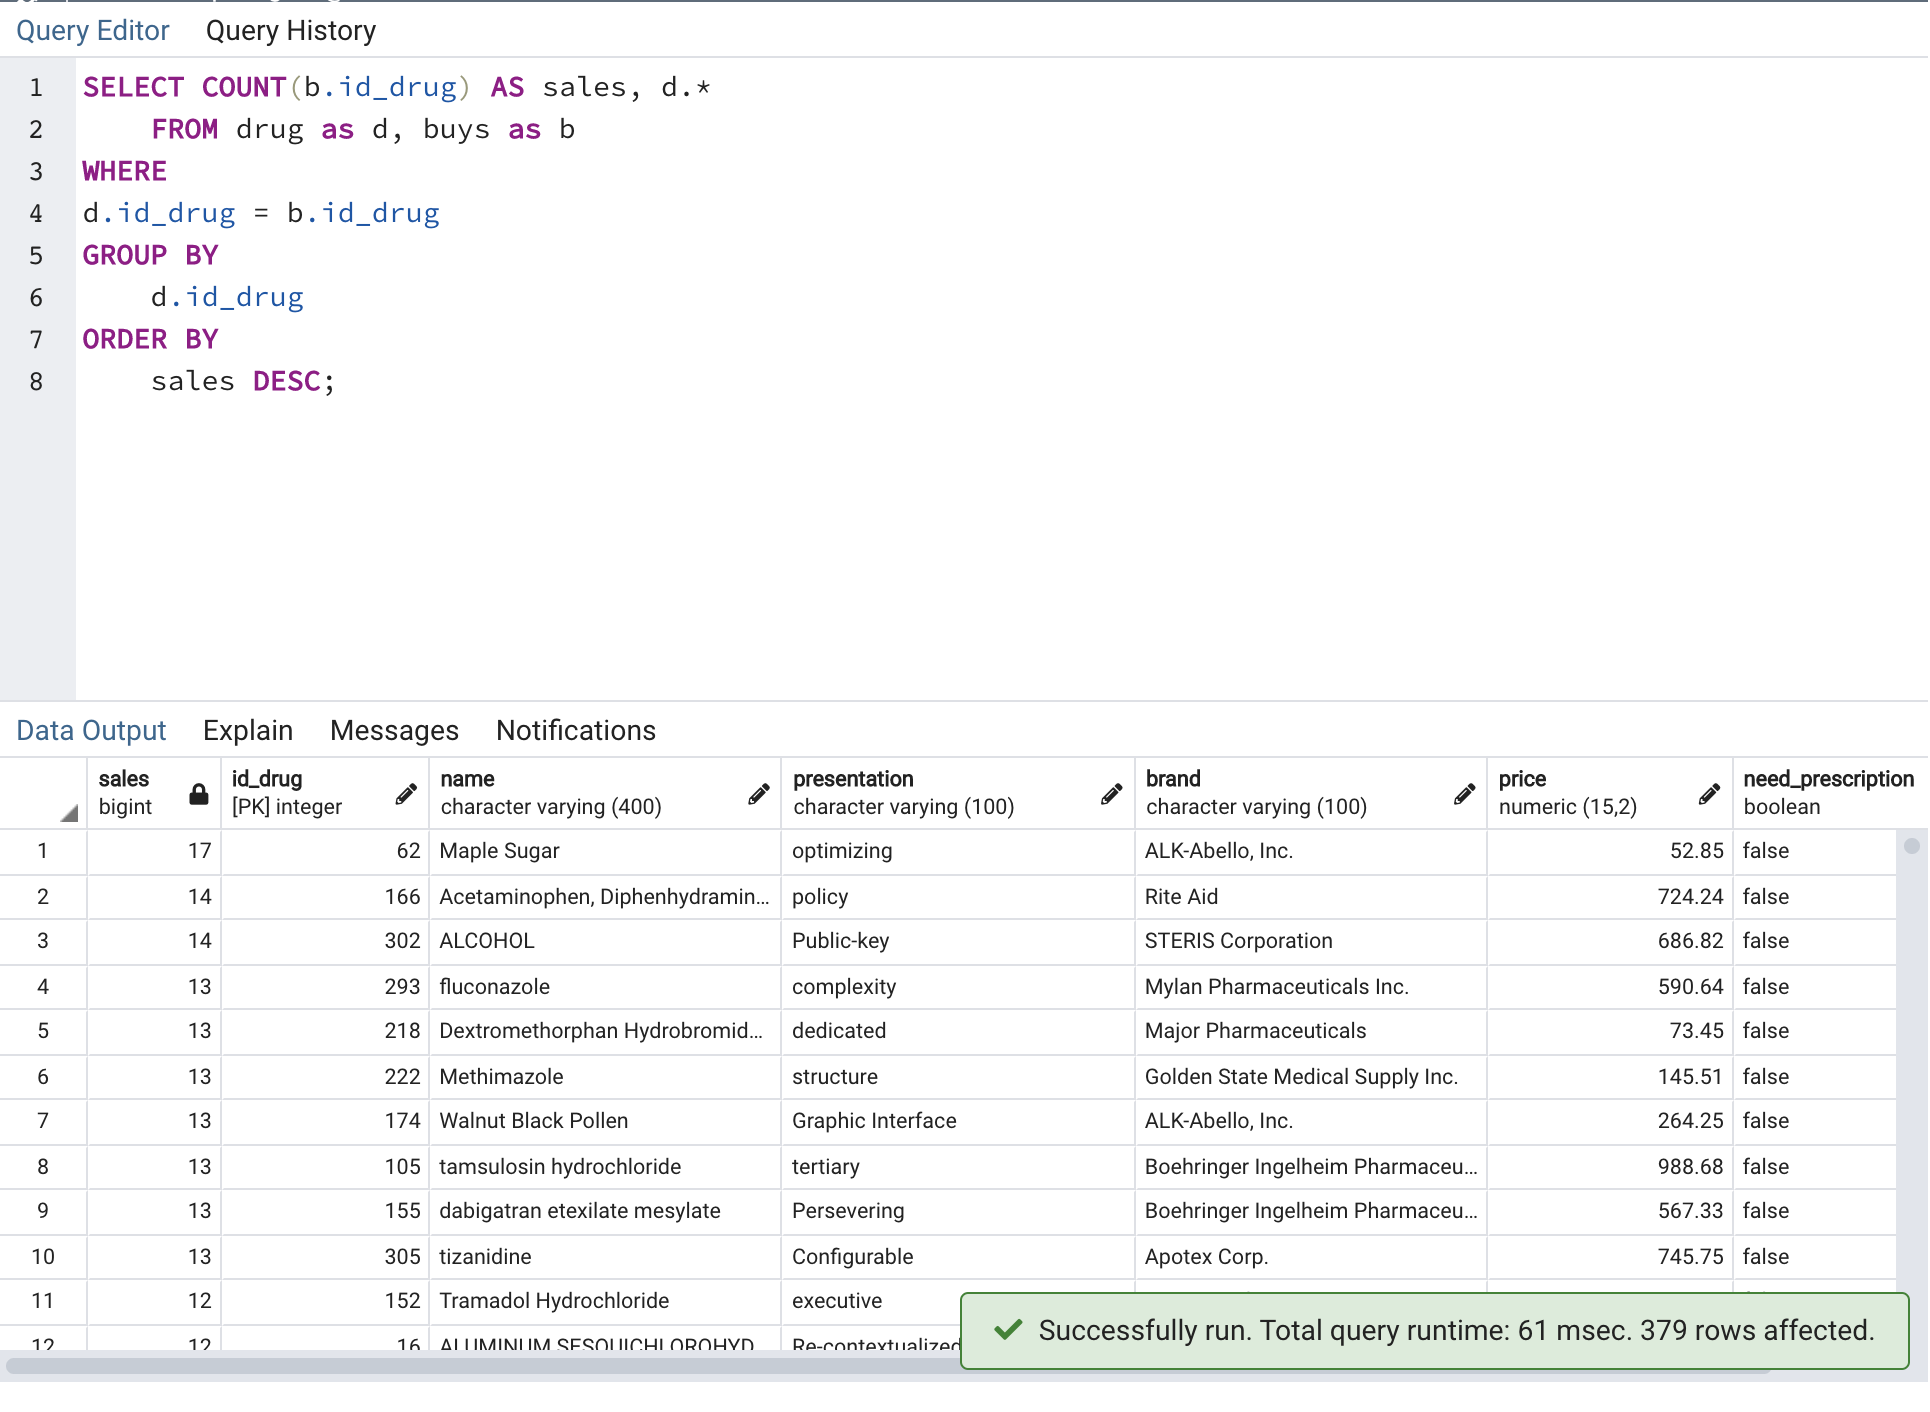
\includegraphics[width=0.9\textwidth]{4}
                \caption{Con nuestra solución podemos tambien saber con información de tiempo real cuales
                son los productos que mas se han vendido (dando detalles que la presentación mas popular por ejemplo)}
            \end{figure}
        
        \clearpage
        \section{Consultas por especialidad}
            
            \begin{figure}[ht]
                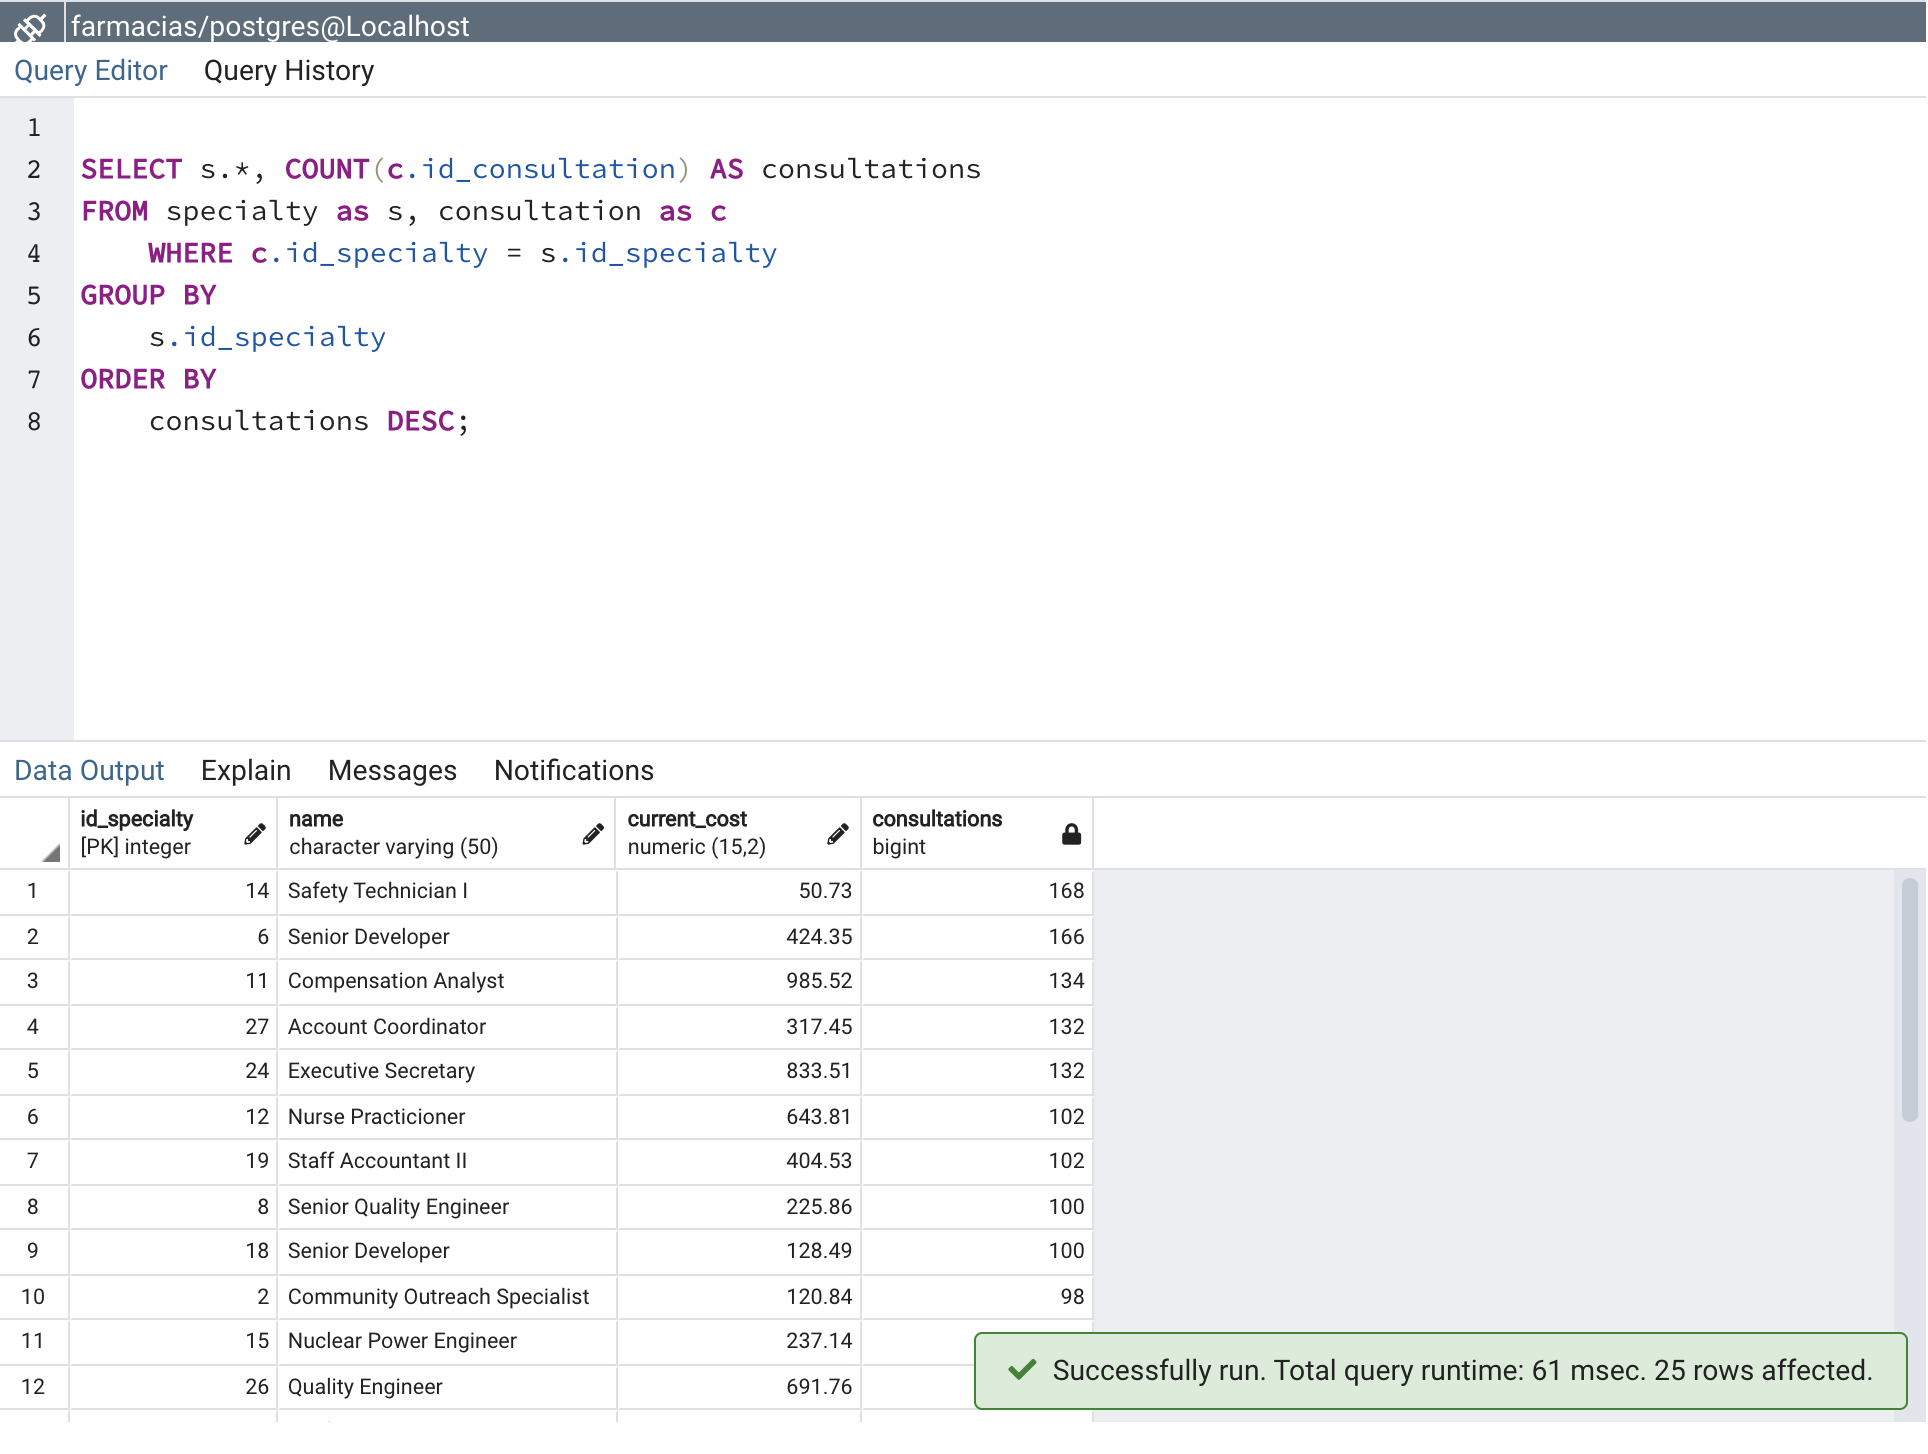
\includegraphics[width=0.9\textwidth]{5}
                \caption{Con nuestra solución podemos tambien cual es el tipo de consulta mas popular y cuando es
                la comision en este momento por dicha especialidad}
            \end{figure}


        \clearpage
        \section{Mayor ingreso por especialidad}
            
            \begin{figure}[ht]
                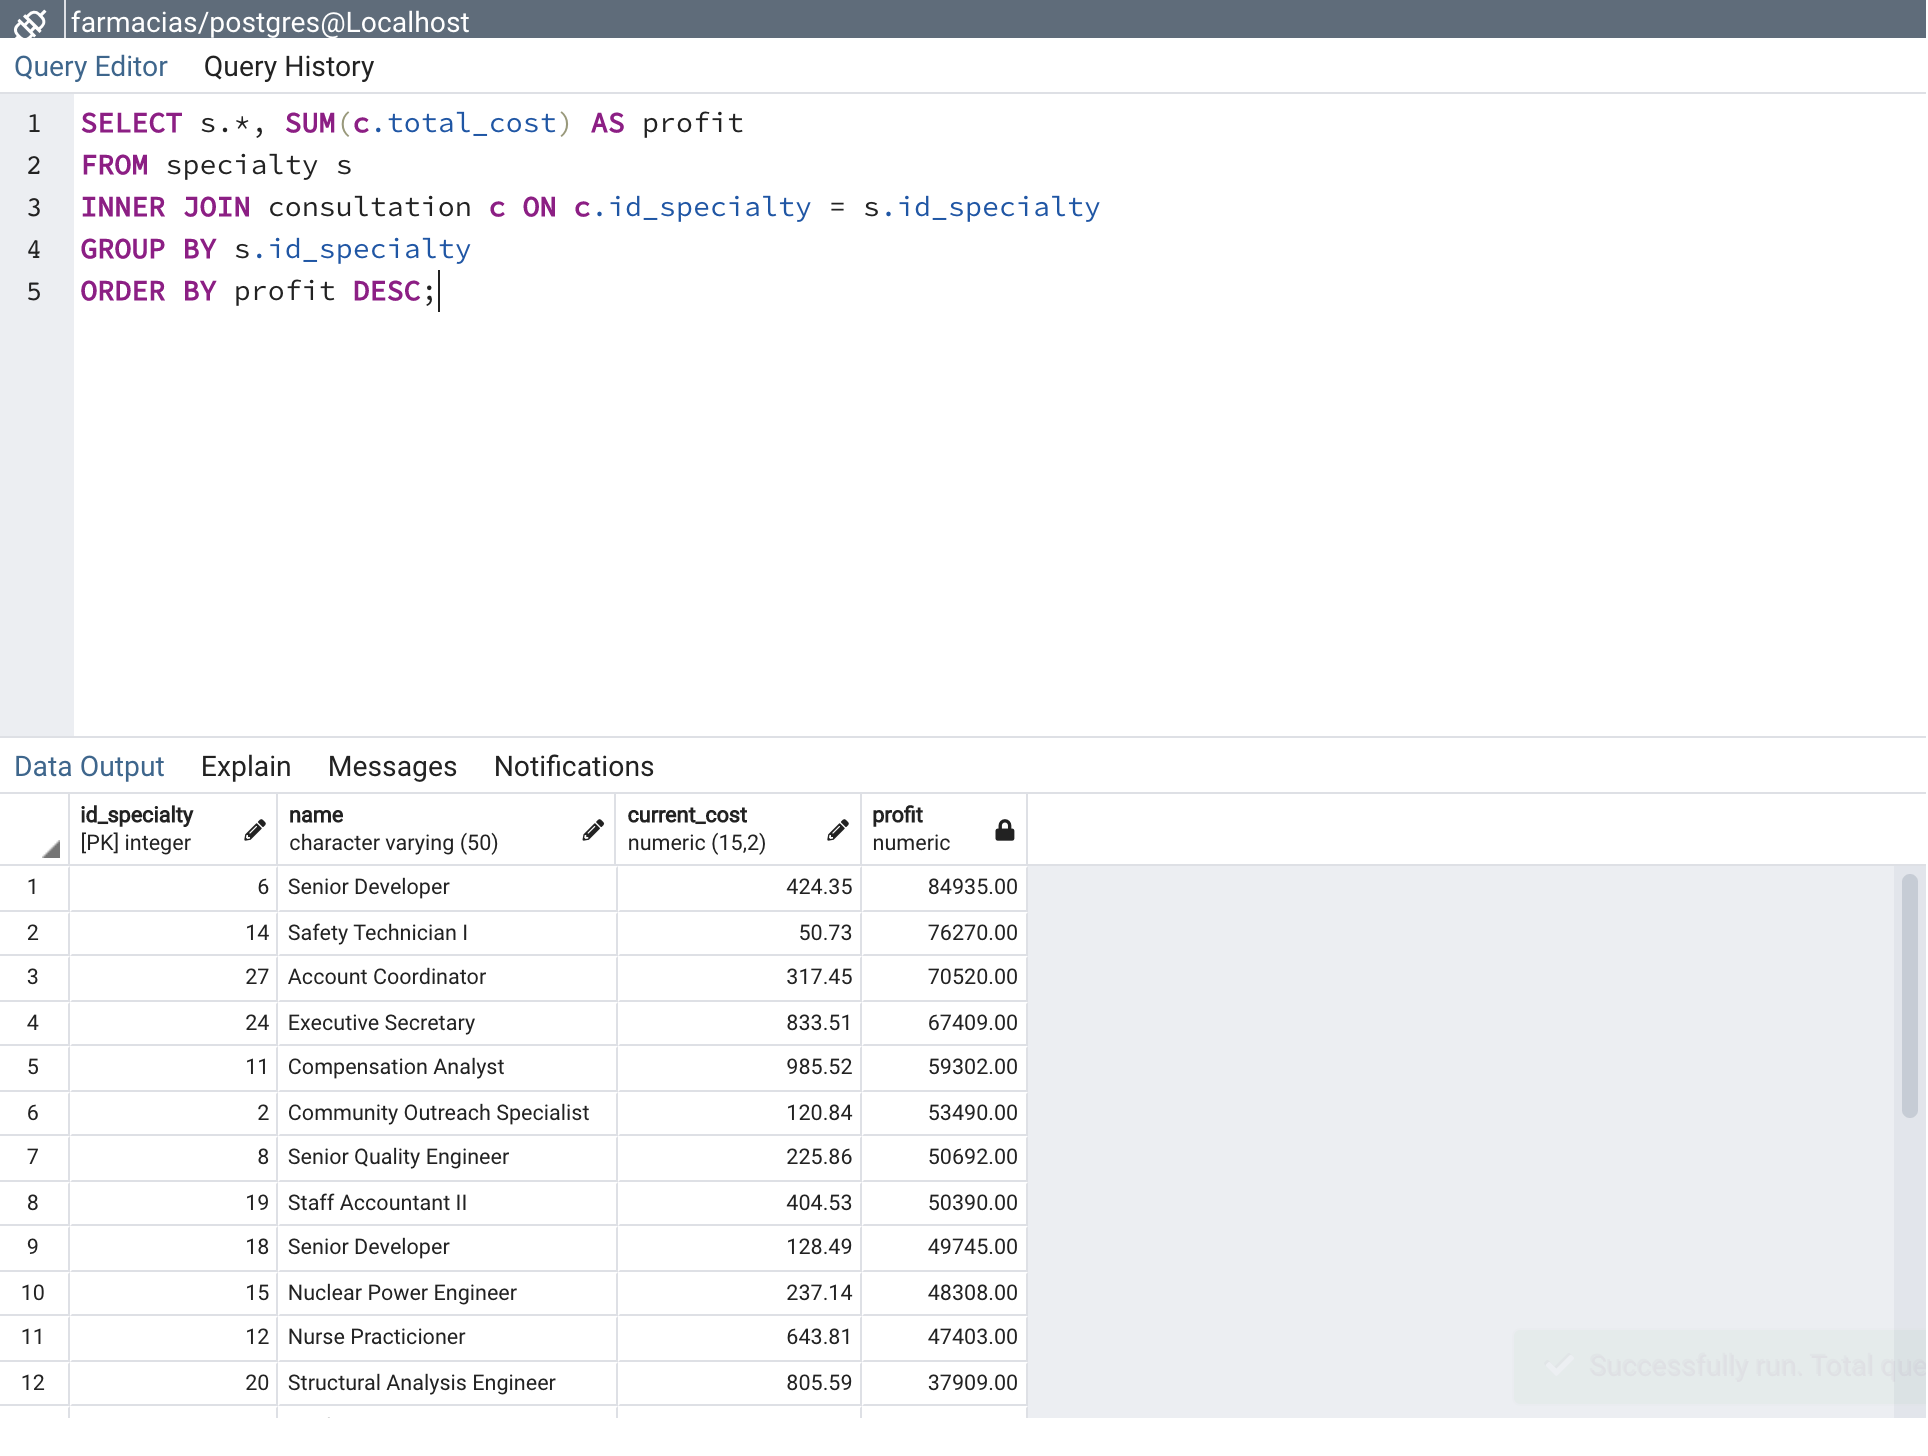
\includegraphics[width=0.9\textwidth]{6}
                \caption{Con nuestra solución podemos ordenar las especialidades basados en la cantidad de ingresos que hemos
                recibido por ellas (es decir sumar la comision de cada consulta hecha de dicha especialidad)}
            \end{figure}

        \clearpage
        \section{Balance promedio entre clientes vs pacientes}
            
            \begin{figure}[ht]
                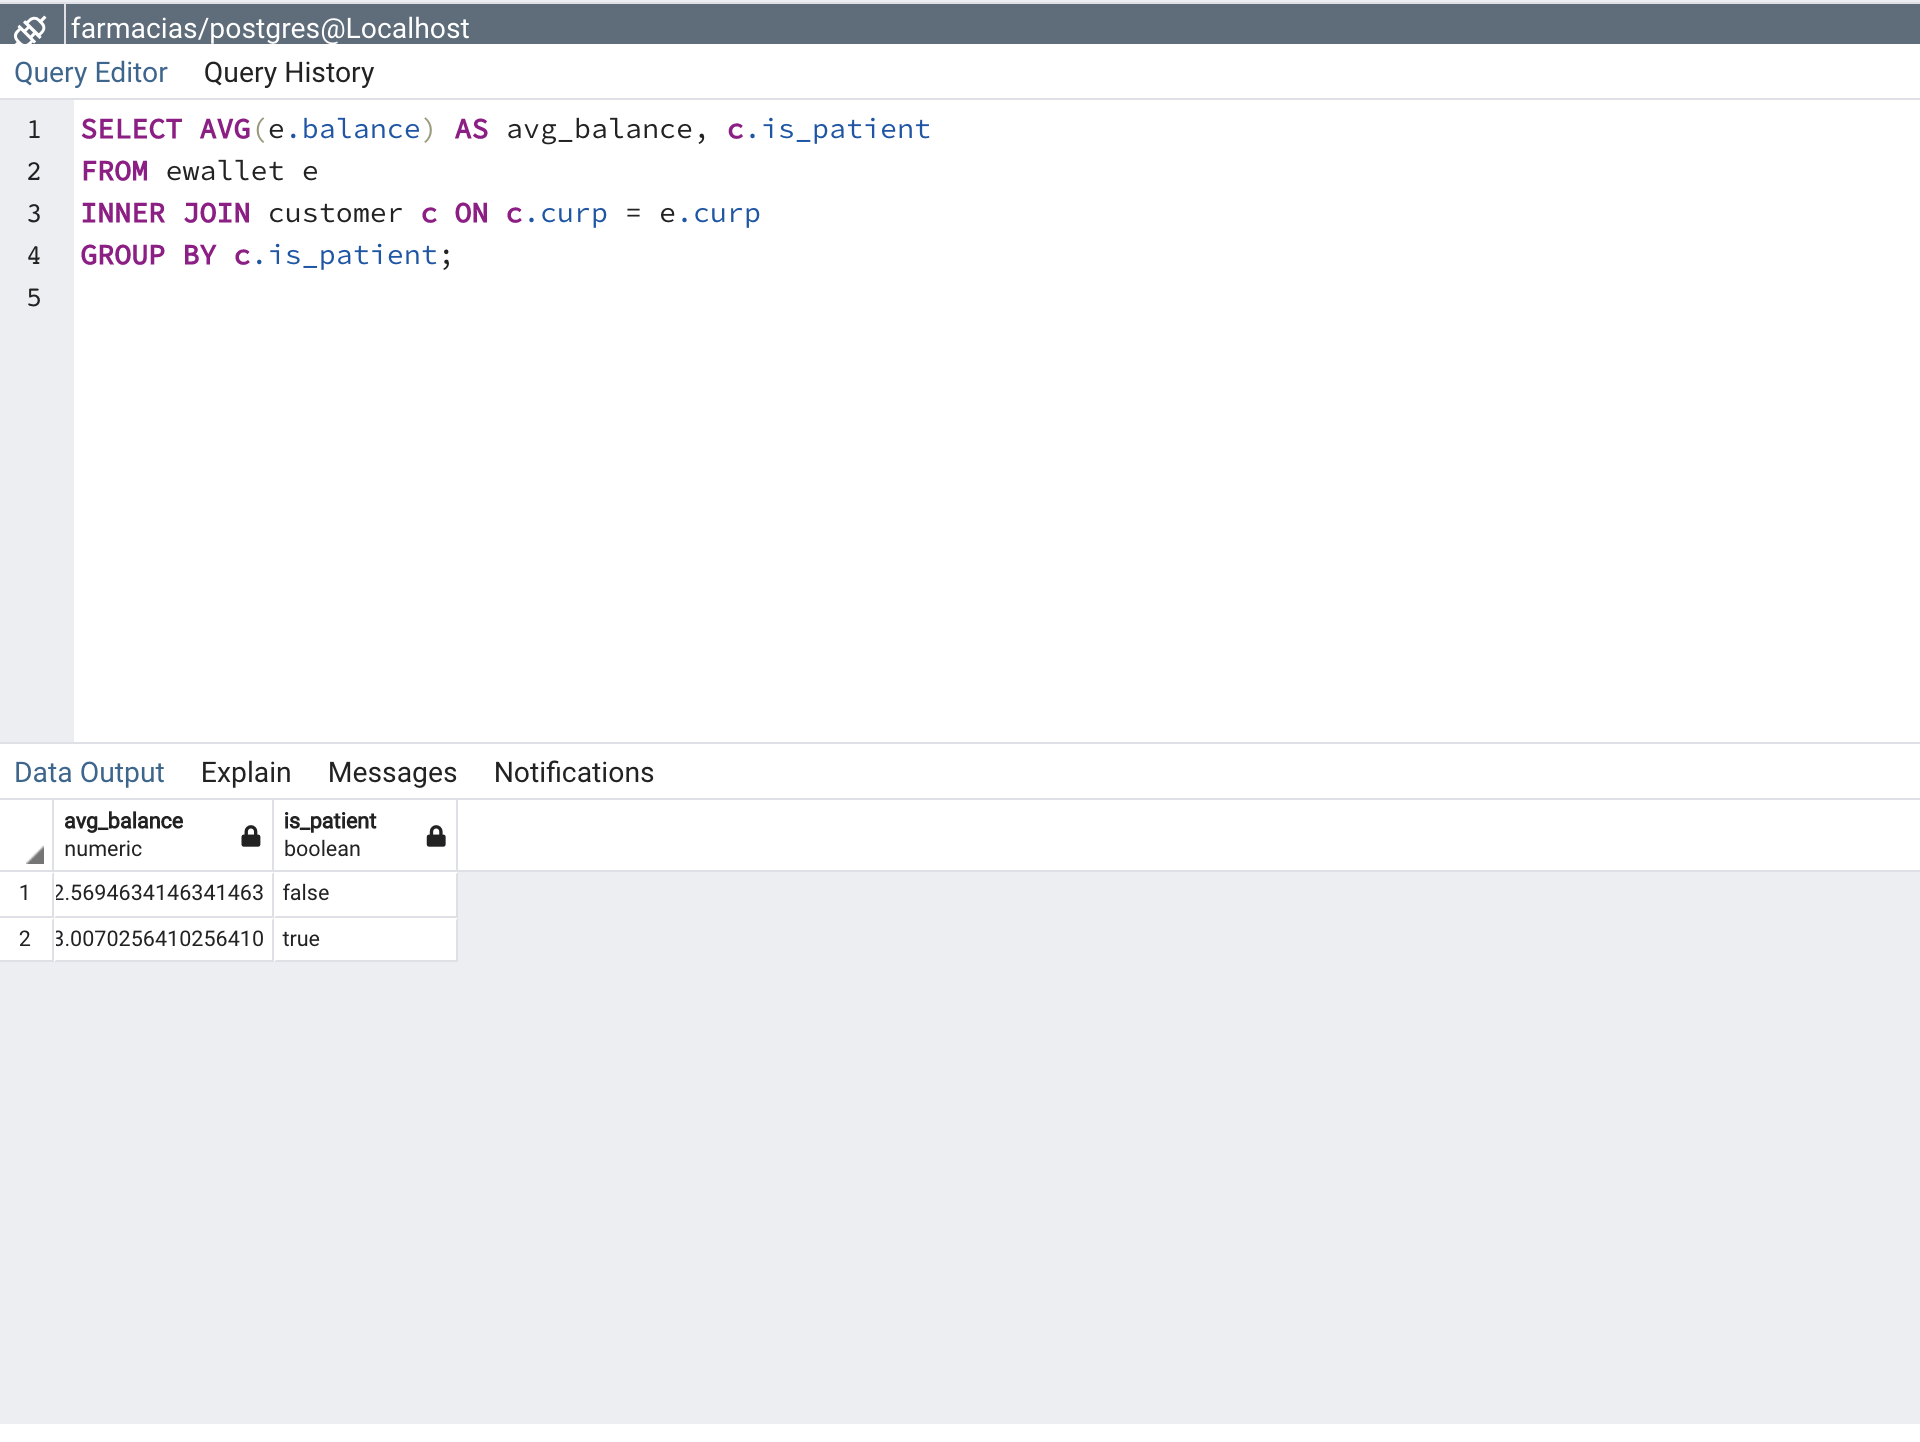
\includegraphics[width=0.9\textwidth]{7}
                \caption{Con nuestra solución podemos tambien usando información en tiempo real saber cual es el balance promedio
                de alguien que solo sea un cliente y alguien que sea un paciente}
            \end{figure}


        \clearpage
        \section{Cajeros mas productivos}
            
            \begin{figure}[ht]
                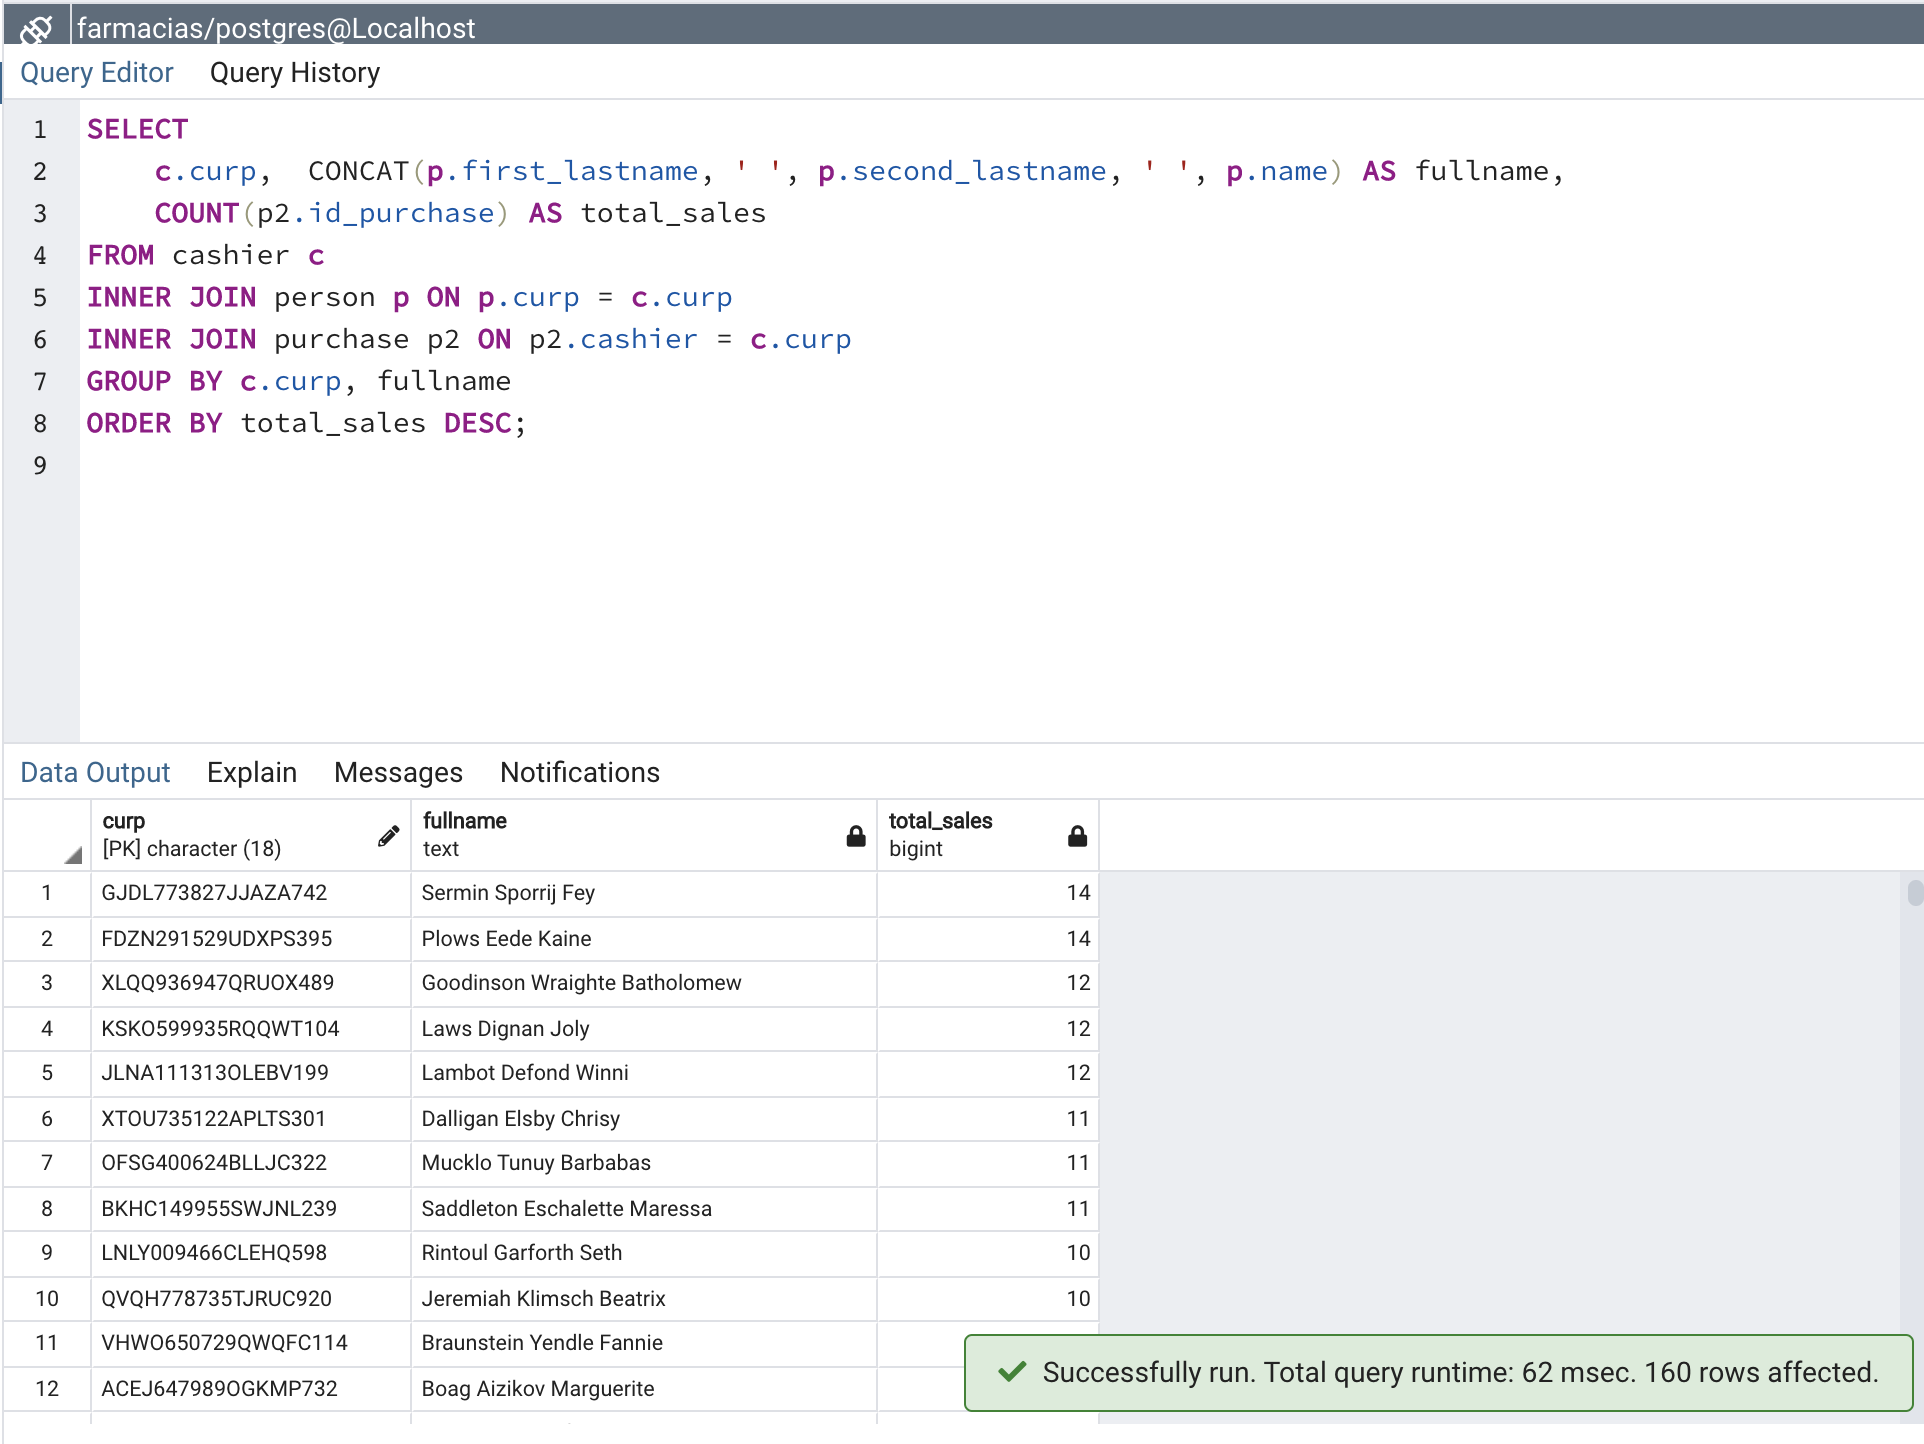
\includegraphics[width=0.9\textwidth]{8}
                \caption{Con nuestra solución podemos saber para cada cajero cuantas ventas ha realizado}
            \end{figure}

        \clearpage
        \section{Ventas por hora}
            
            \begin{figure}[ht]
                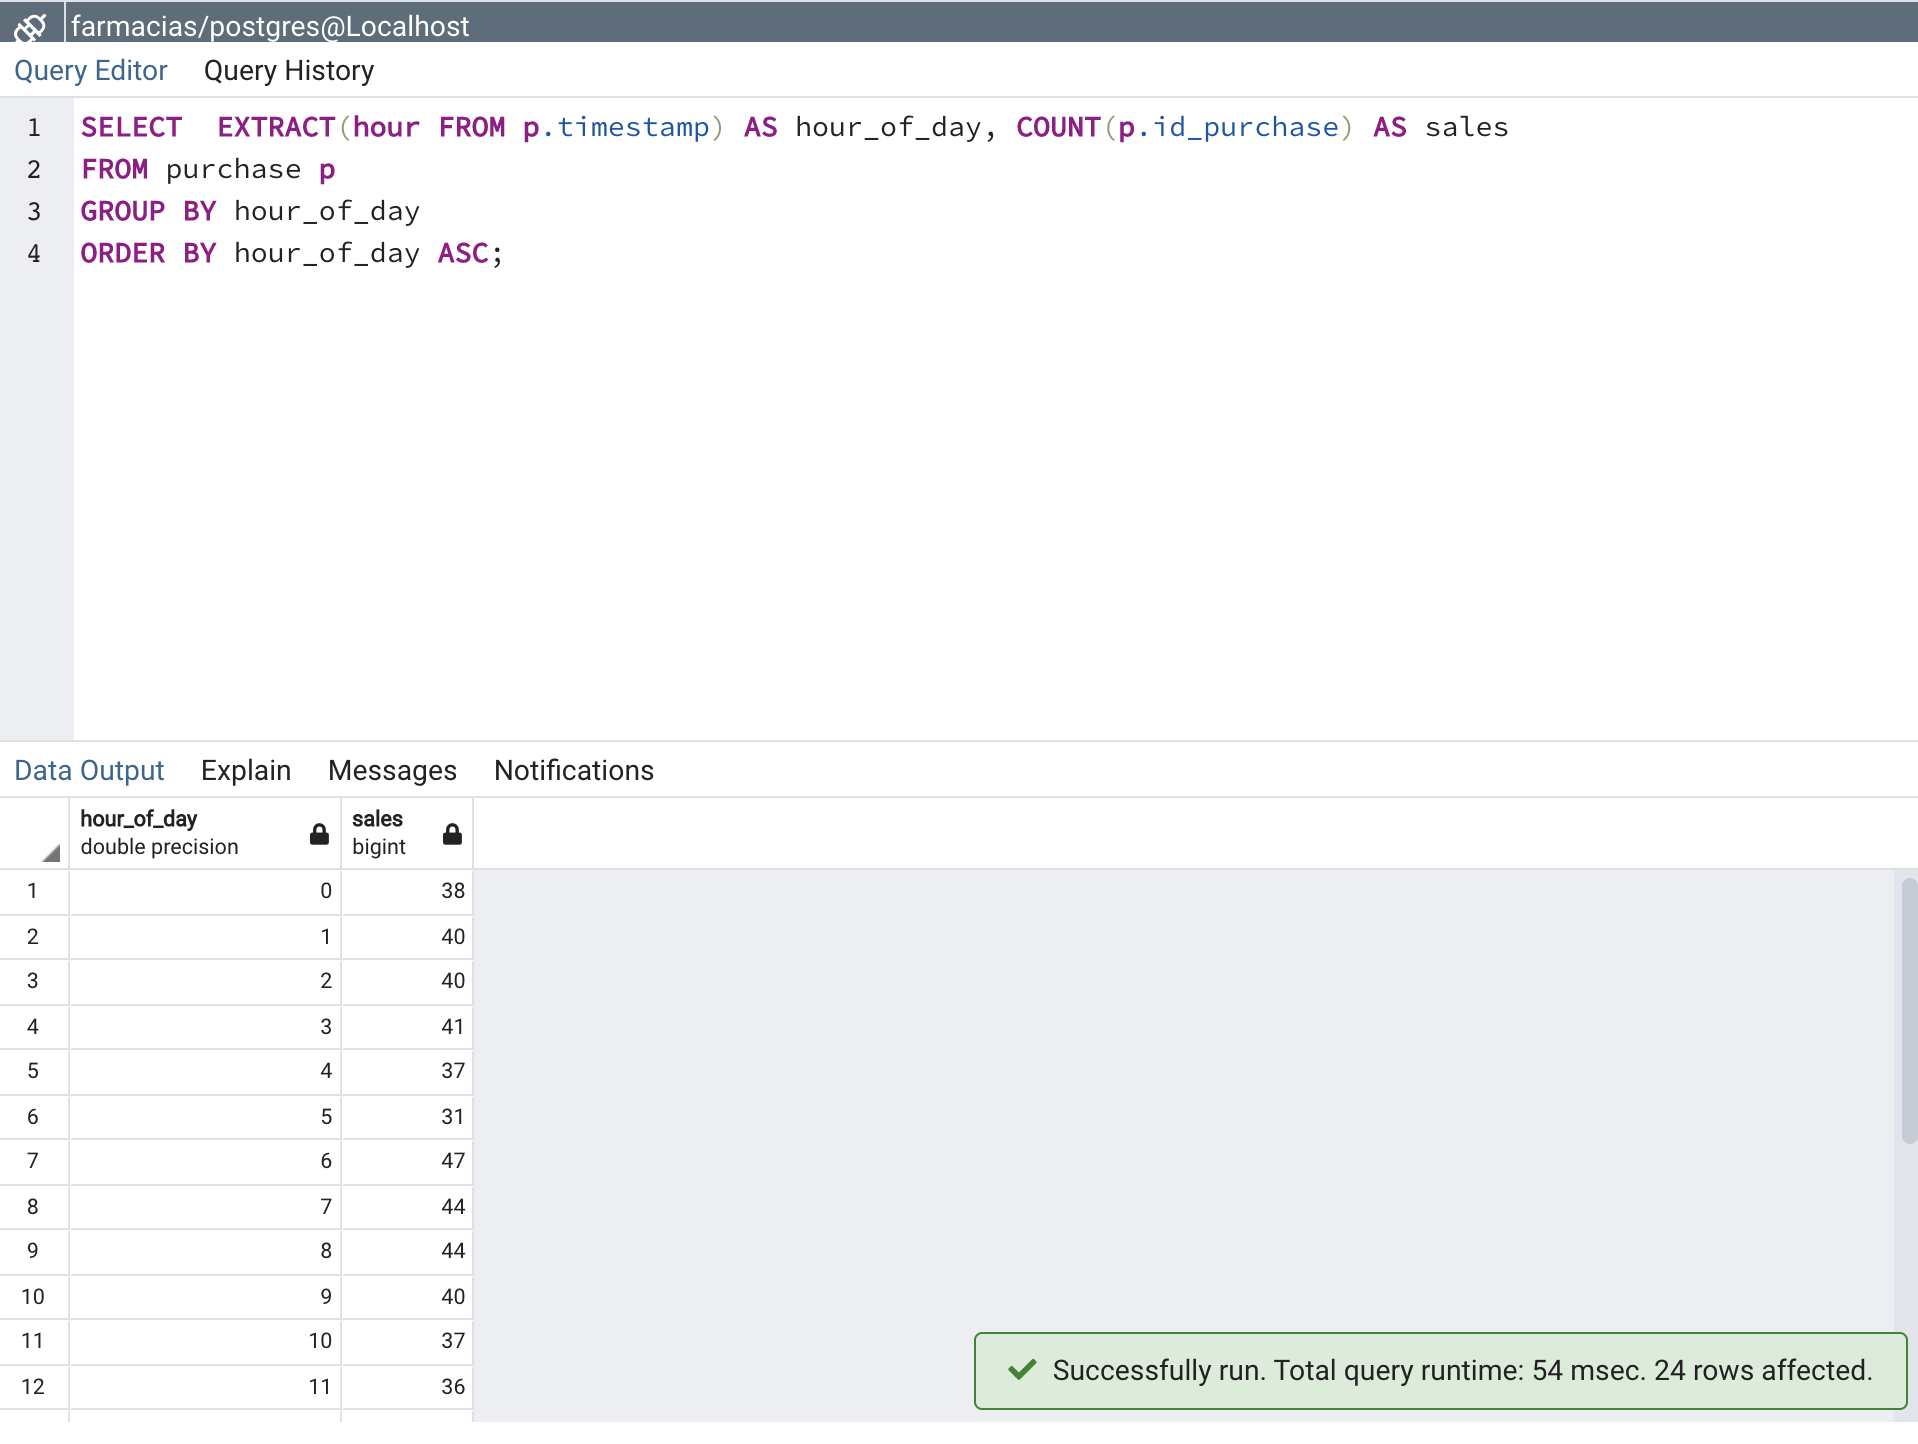
\includegraphics[width=0.9\textwidth]{9}
                \caption{Con nuestra solución de manera similar a como hicimos con los meses del año podemos
                ver como fluctuan las venta a lo largo de la hora del día en tiempo real}
            \end{figure}

        \clearpage
        \section{Cuentas de doctores que generan una proxima cita}
            
            \begin{figure}[ht]
                
\includegraphics[width=0.9\textwidth]{10}
                \caption{Con nuestra solución podemos saber rapidamente quieres son los doctores que tienen en este
                momento una cita pendiente}
            \end{figure}

        \clearpage
        \section{Total de medicamentos en receta por especialidad cuyo precio es mayor a 500}
            
            \begin{figure}[ht]
                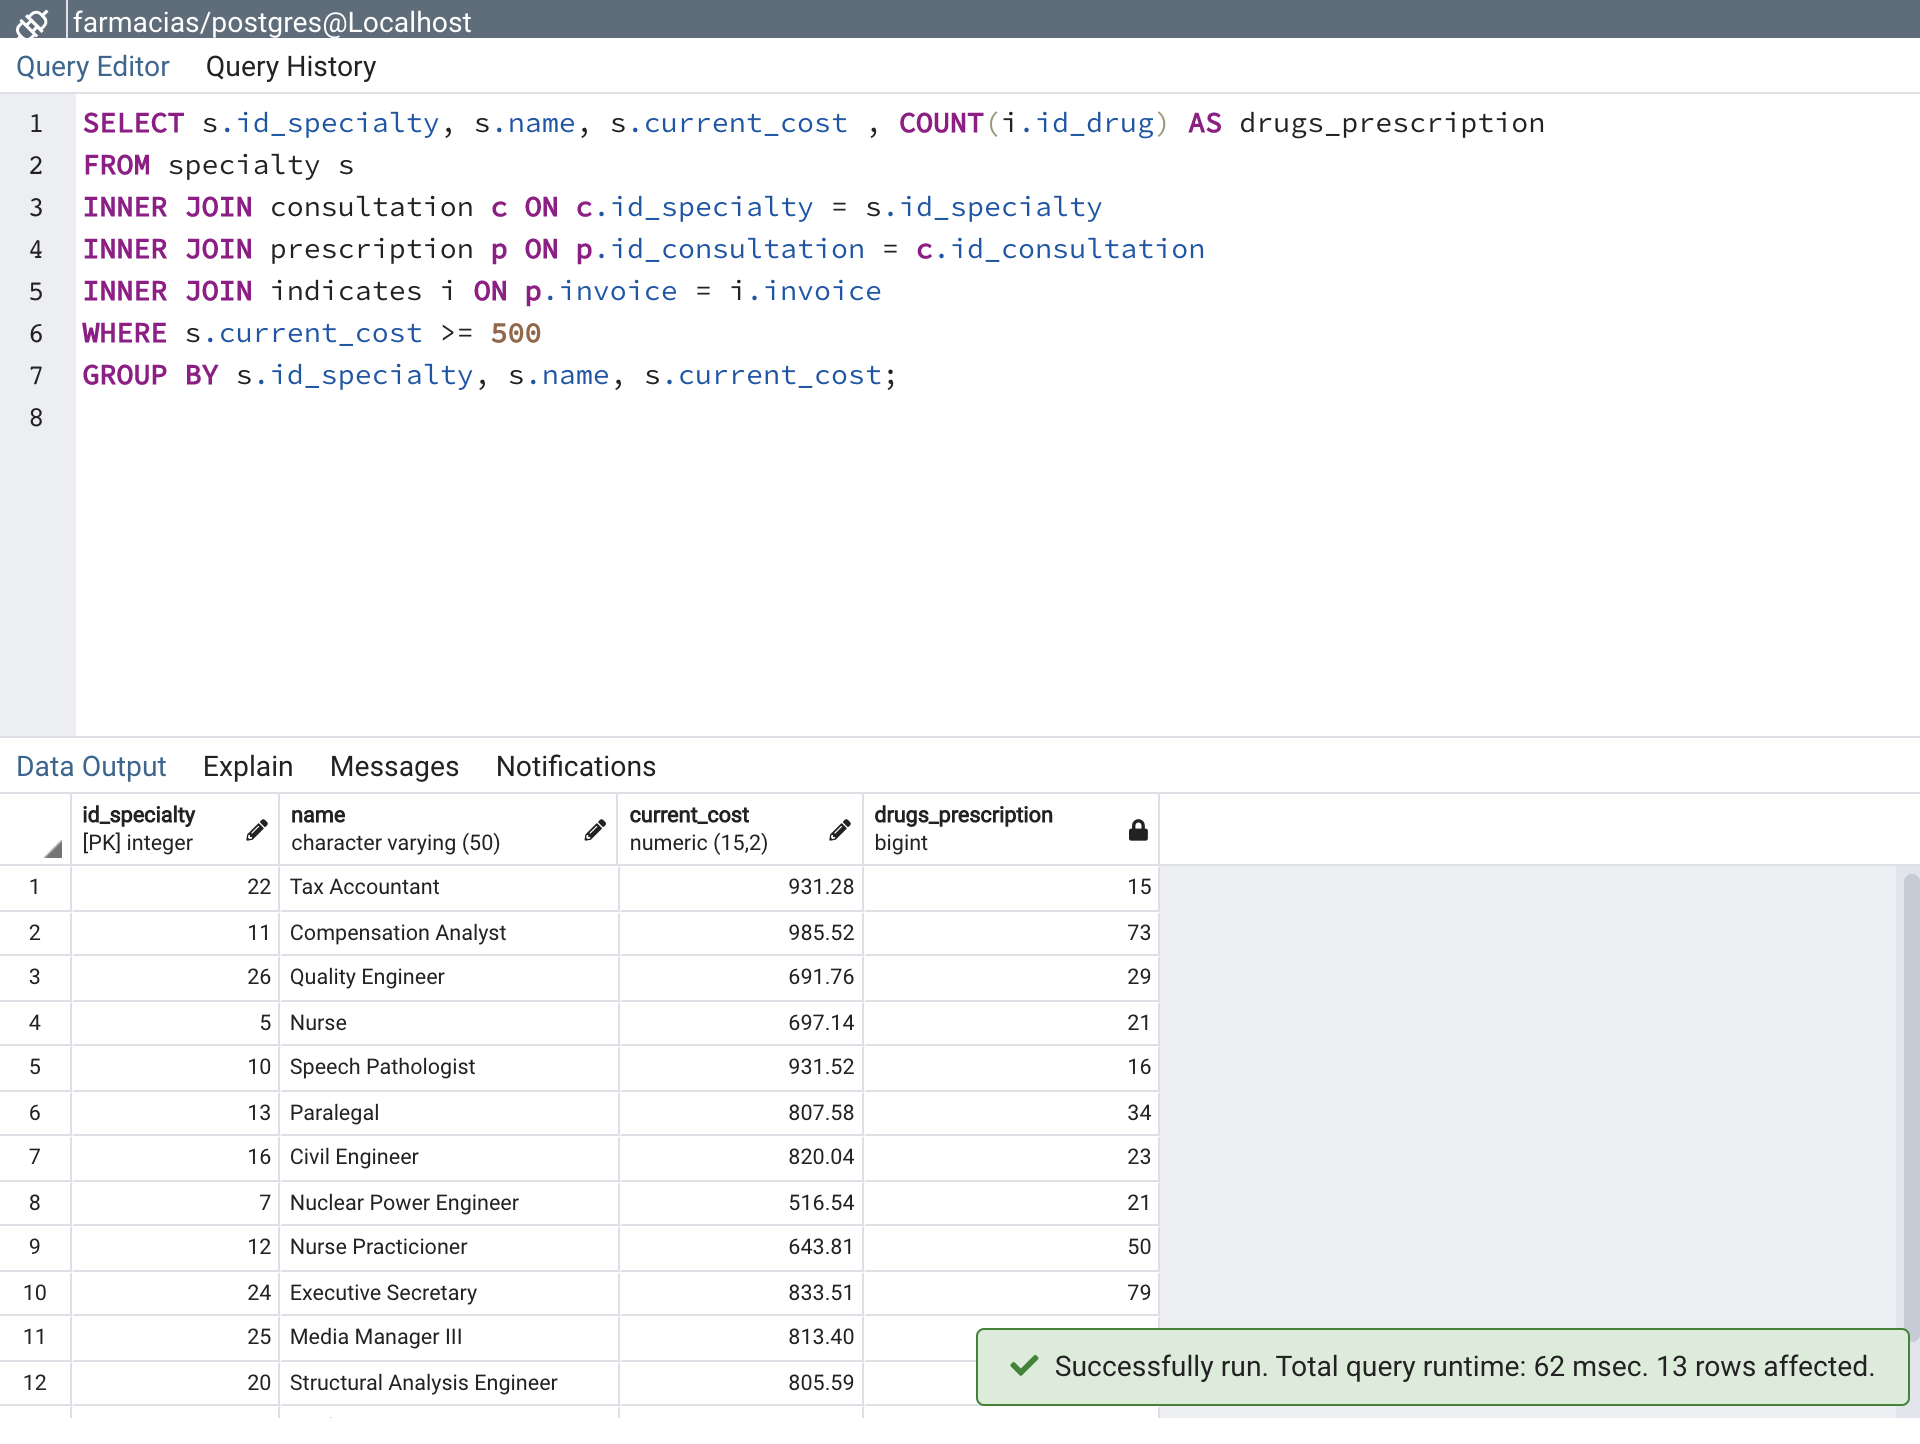
\includegraphics[width=0.9\textwidth]{11}
                \caption{aqui por ejemplo podemos ver los medicamentos que requieren receta que provienen de una
                cita por especialidad que costo mas de 500, ademas mostramos cuantas veces dicho medicamente ha sido
                comprado
                }
            \end{figure}
    

        \clearpage
        \section{Posible ingreso por farmacos que vengan por receta}
            
            \begin{figure}[ht]
                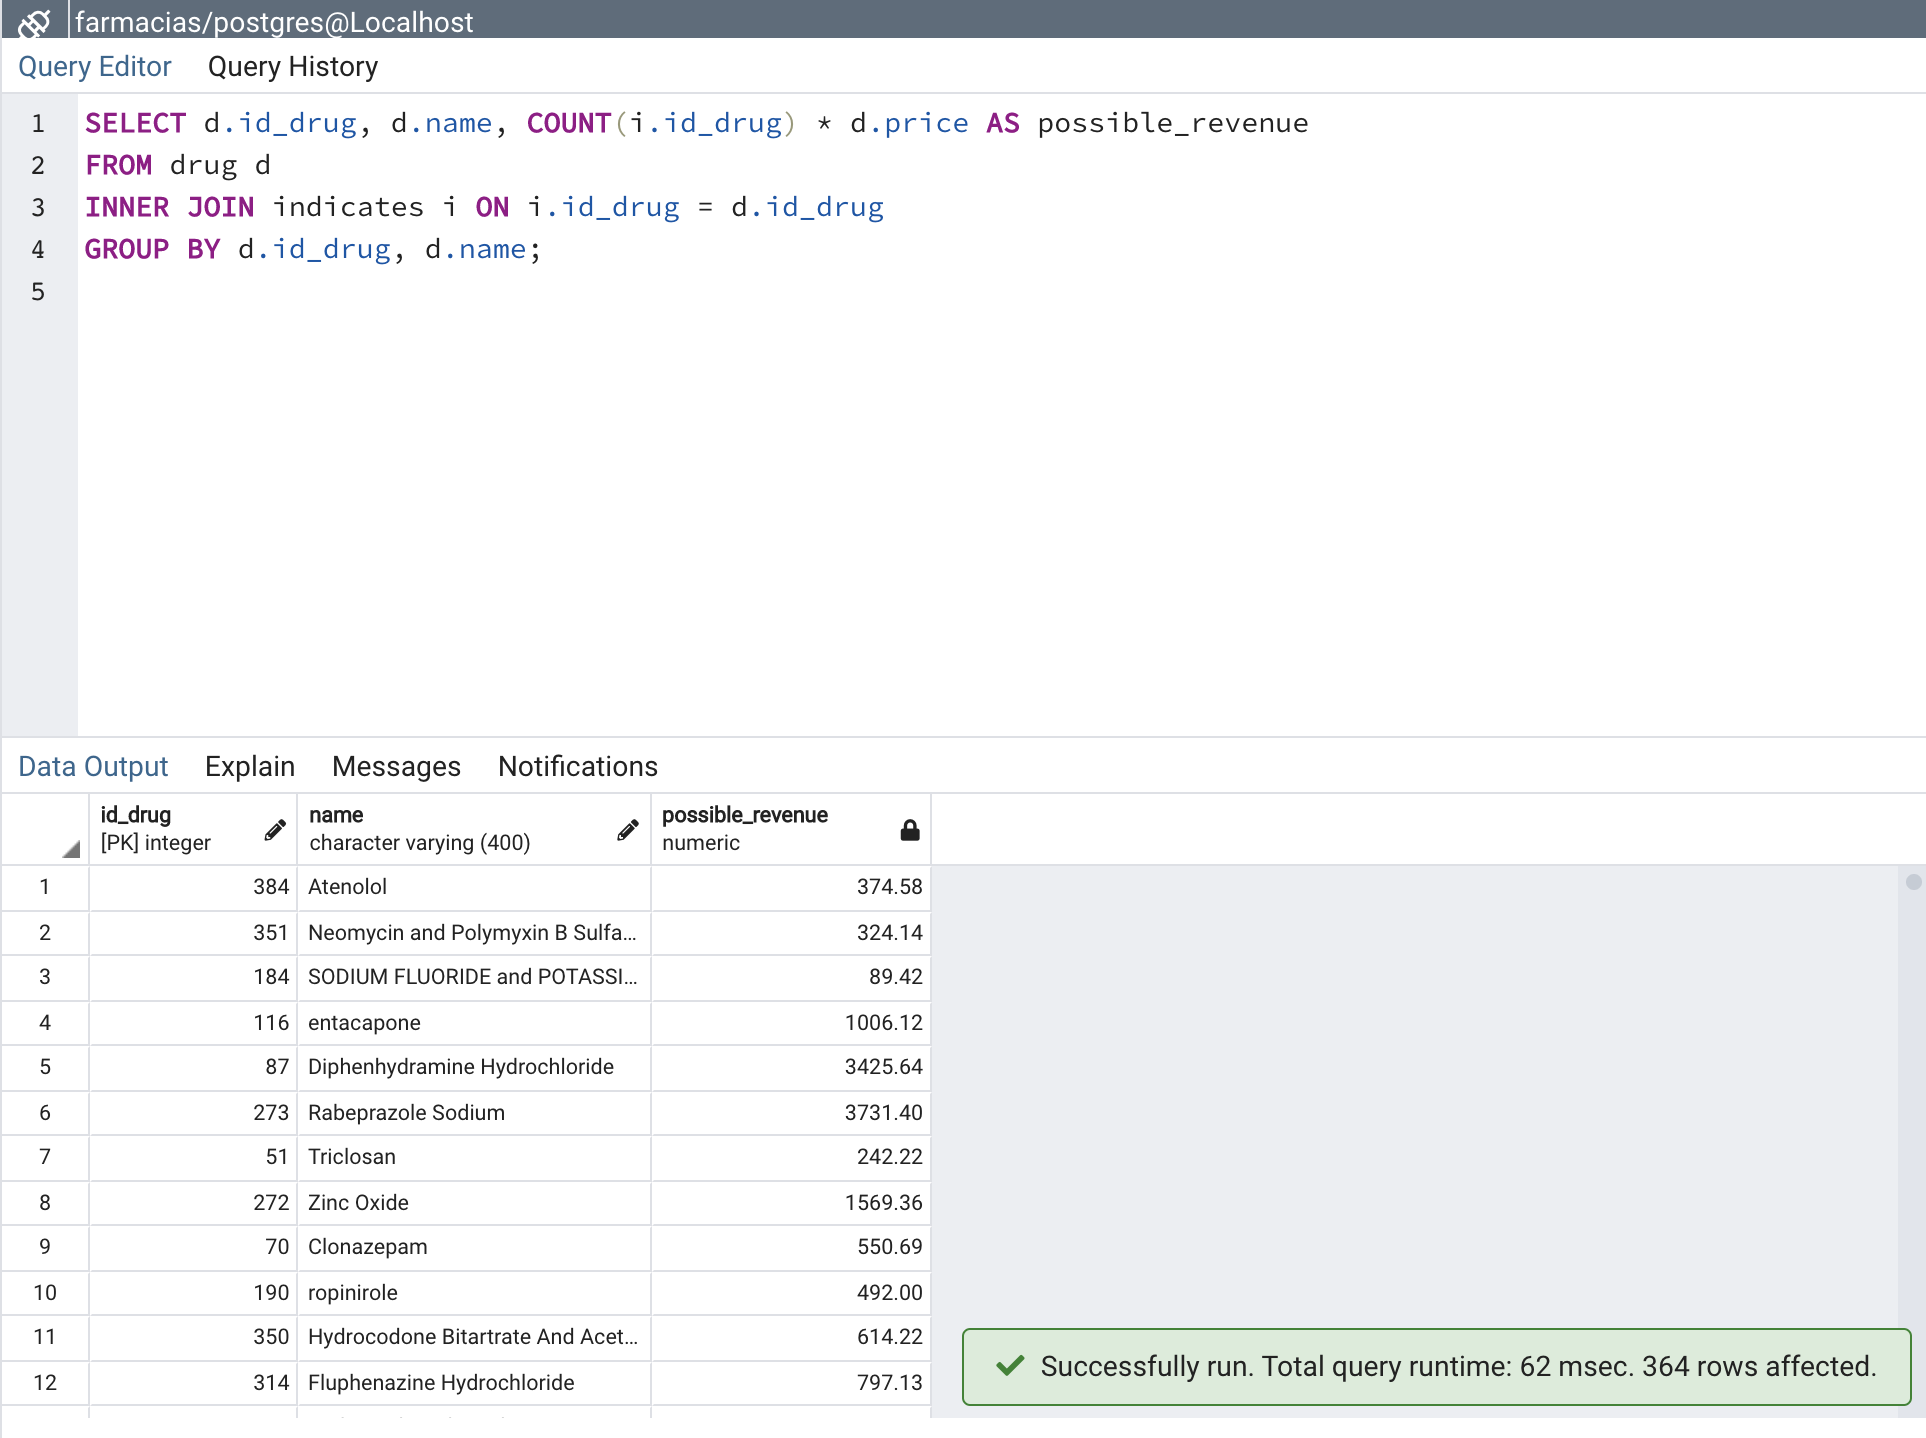
\includegraphics[width=0.9\textwidth]{12}
                \caption{aqui podemos ver los ingresos que hemos tenido debido a medicamentos que provienen 
                de una prescripción
                }
            \end{figure}
    
        \clearpage
        \section{Demografica de nuestros pacientes}
            
            \begin{figure}[ht]
                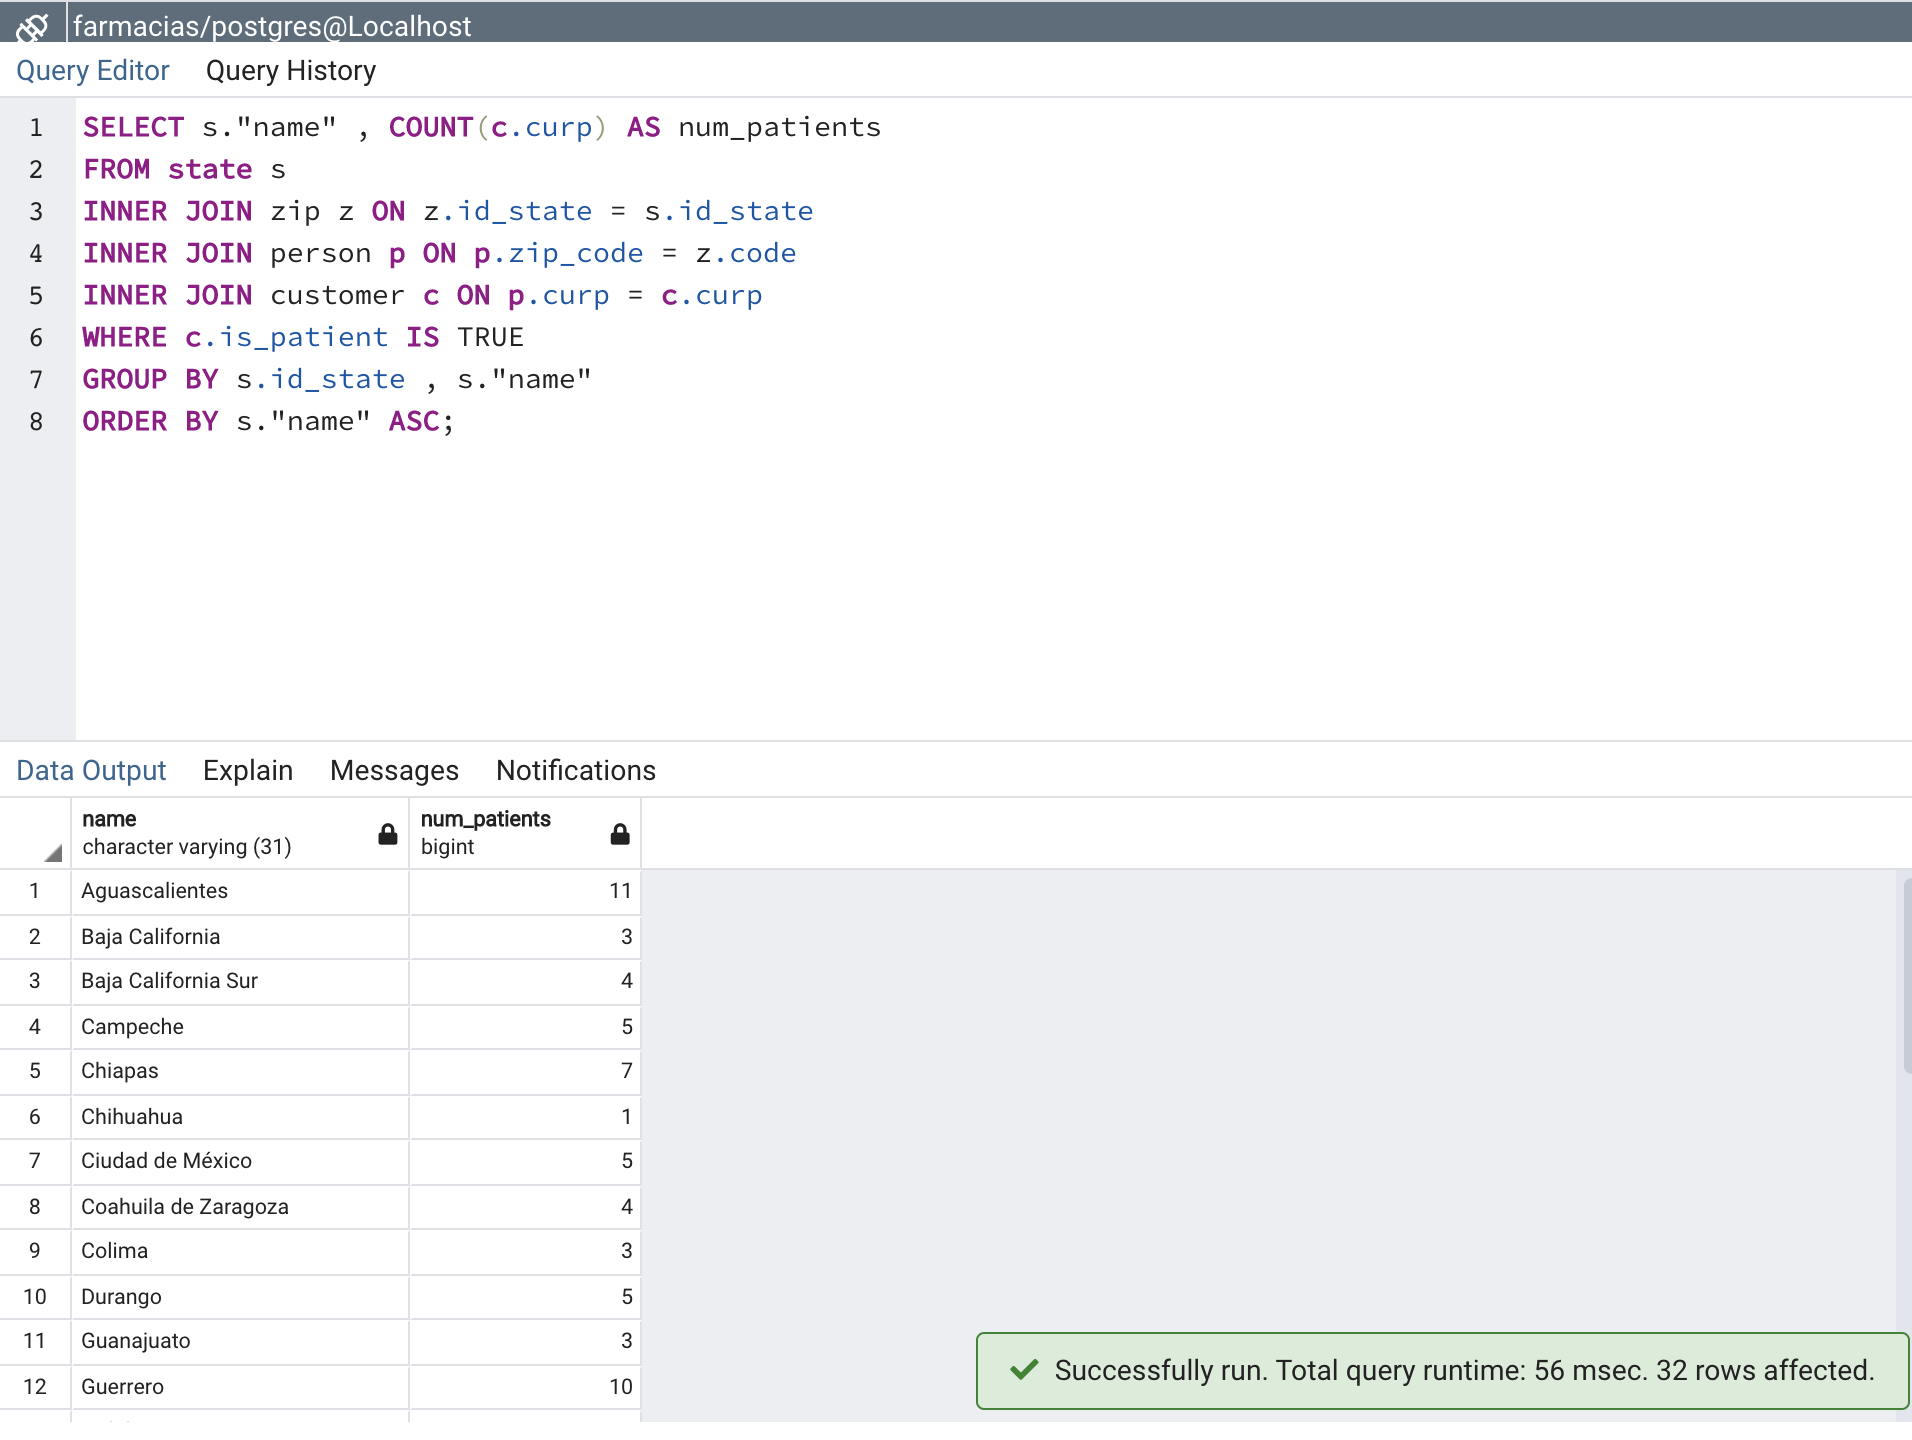
\includegraphics[width=0.9\textwidth]{13}
                \caption{aqui podemos la cantidad de pacientes que atendemos por estado de origen
                }
            \end{figure}

        \clearpage
        \section{La ubicación por estado que genera más ingreso a través de compras por clientes}
            
            \begin{figure}[ht]
                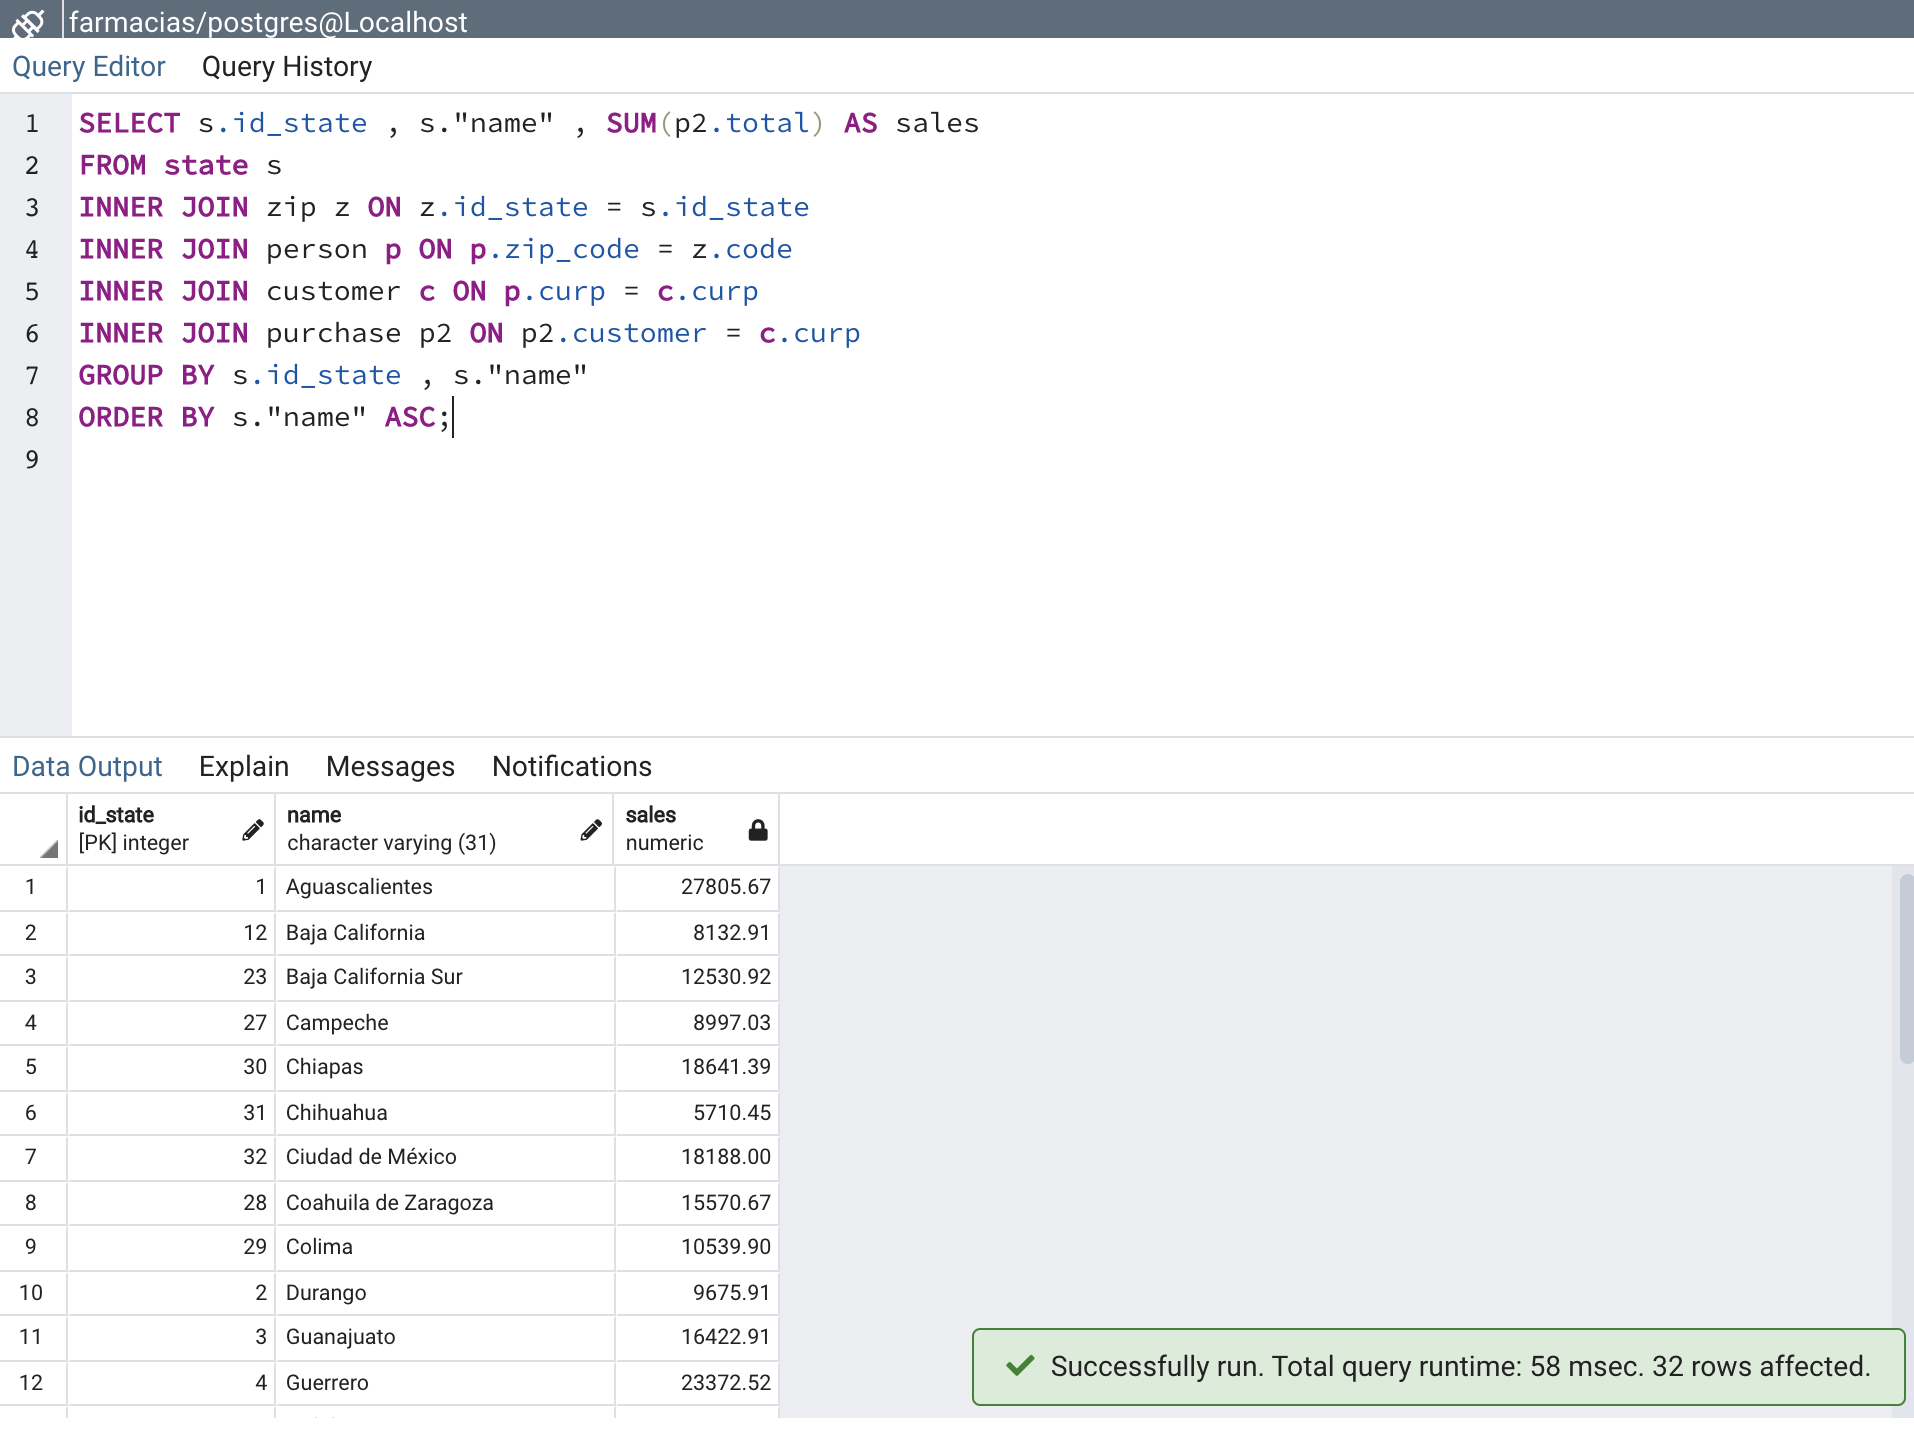
\includegraphics[width=0.9\textwidth]{14}
                \caption{La ubicación por estado que genera más ingreso a través de compras por clientes
                }
            \end{figure}  


        \clearpage
        \section{Ventas de fármacos que necesitan receta}
            
            \begin{figure}[ht]
                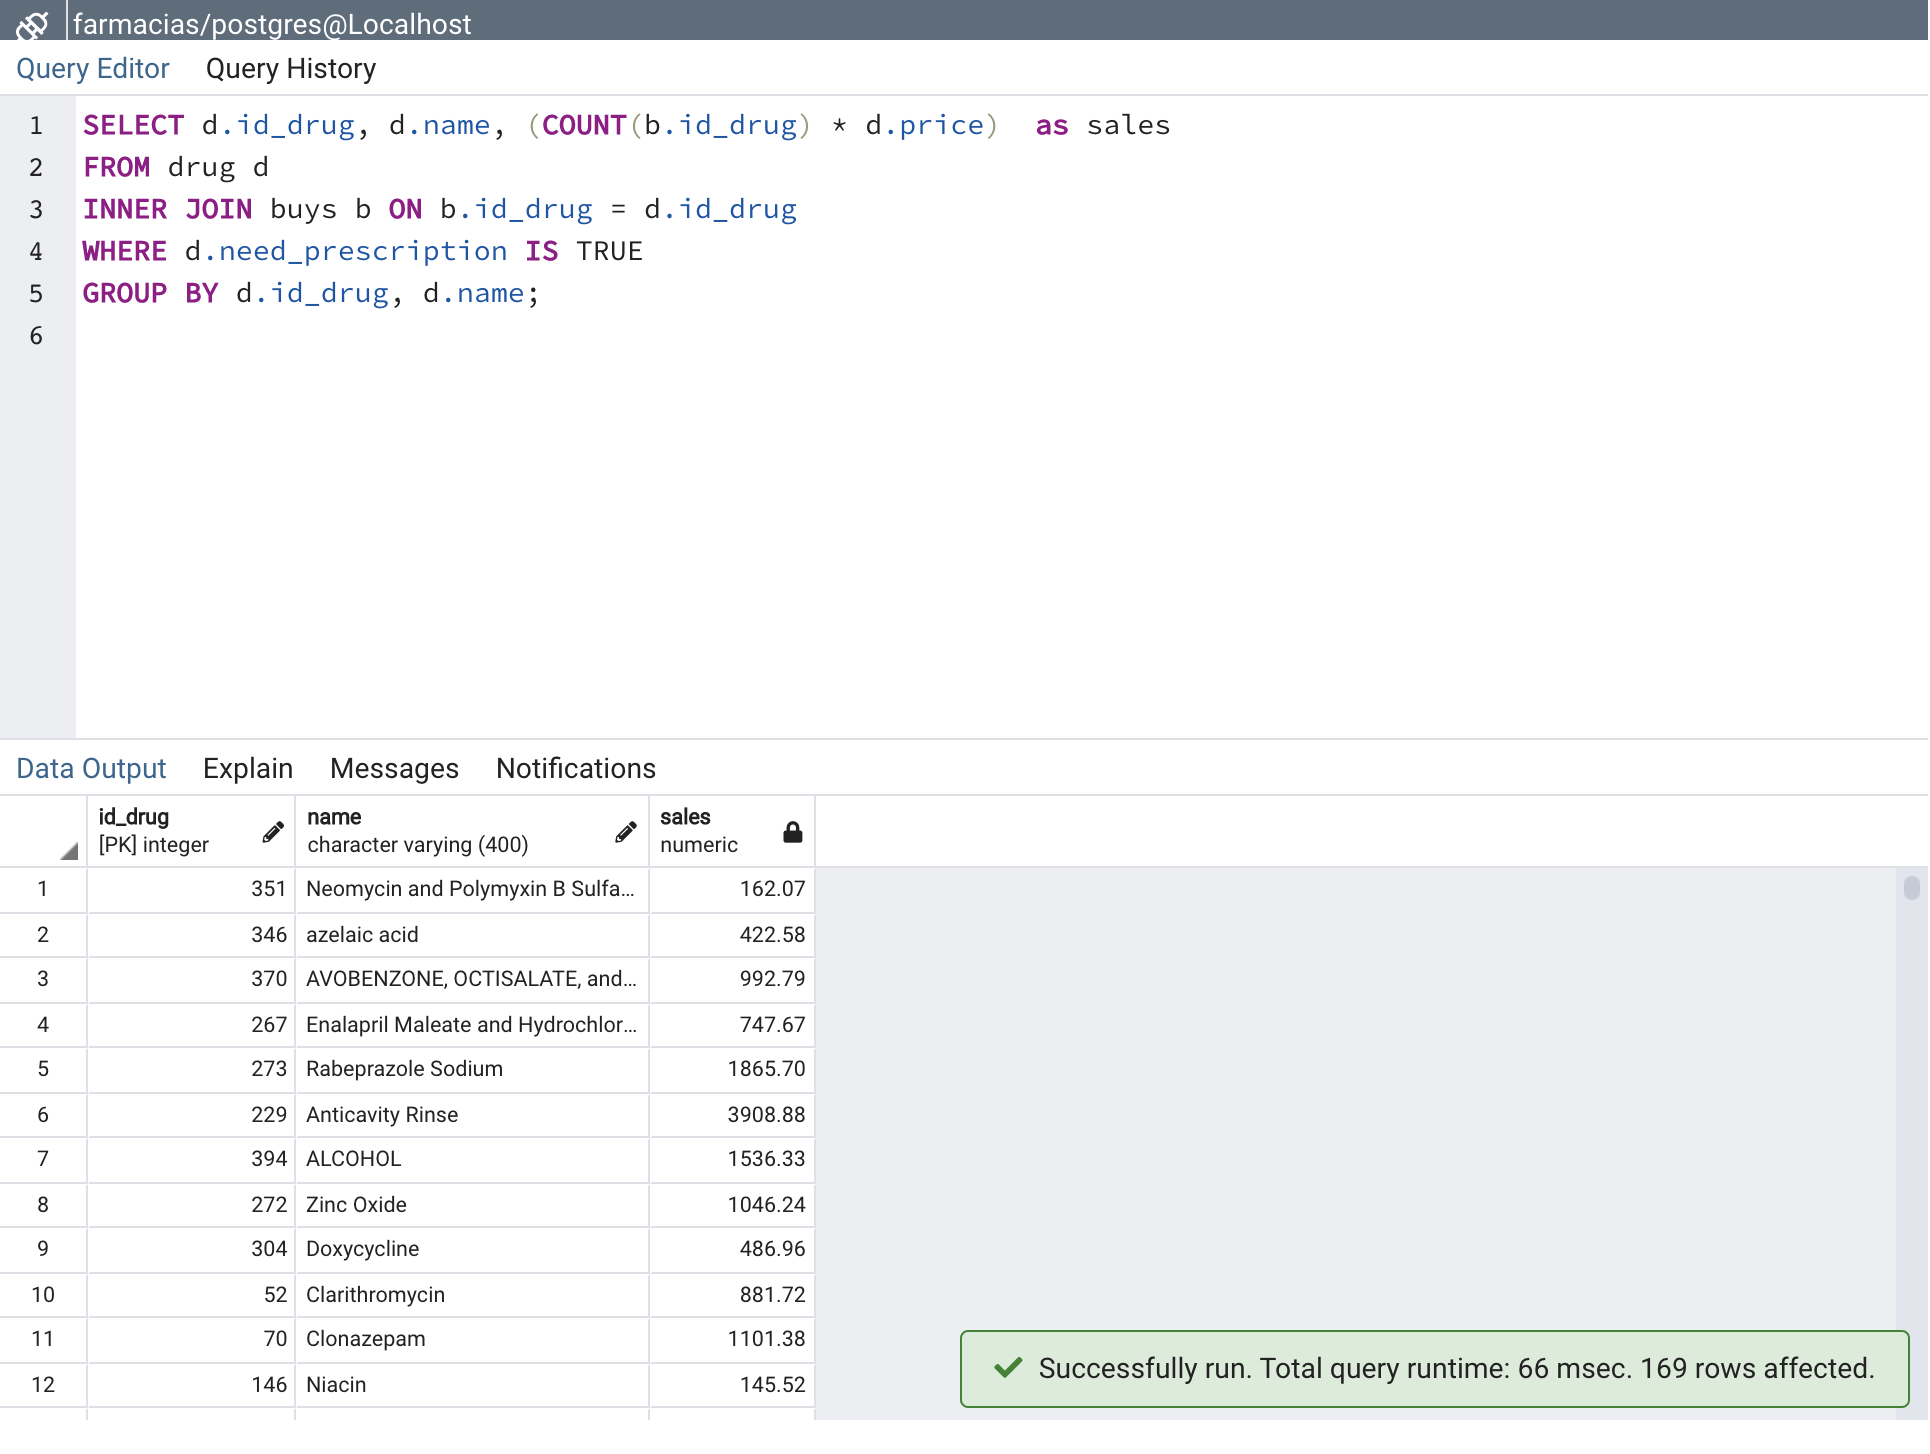
\includegraphics[width=0.9\textwidth]{15}
                \caption{Aqui podemos ver las ventas de los medicamentos en los que es necesaria una receta para
                su venta
                }
            \end{figure}  

\end{document}